% ============================================================
% 主文档 main.tex —— 编译整本书时使用本文件
% ============================================================
% 魔术注释(供编辑器识别编译方式):
% !TEX program = xelatex
% !TEX encoding = UTF-8
% ============================================================
% 中文书籍模板(ctexbook)
% 编译方式: 使用 XeLaTeX 或 LuaLaTeX 编译(推荐 XeLaTeX)。
% 该模板默认自动选用系统可用的中文字体,如需指定可加选项,如:
%   \documentclass[11pt,a4paper,fontset=fandol]{ctexbook}
% ============================================================
% 文件结构说明:
%   main.tex             本文件: 全书骨架(封面/目录/前言/分篇/引入各章)
%   preamble.tex         共享导言区: 宏包与样式, 整书和各章共用
%   ch01-ubuntu-ros.tex       第 1 章 Ubuntu 与 ROS 简介
%   ch02-ubuntu-commands.tex  第 2 章 Ubuntu 常用指令
% ============================================================
% 新增章节方法:
%   1. 复制 ch01 的文件头格式, 新建 chNN-xxx.tex, 章标题写在文件内;
%   2. 在下方对应的 \part 之后加一行 \input{chNN-xxx};
%   3. 每个章节文件都可单独编译, 也可随 main.tex 编译整书。
% ============================================================
\documentclass[12pt,a4paper]{ctexbook}
% ============================================================
% 共享导言区 preamble.tex
% 本文件被 main.tex(整书编译)和各章文件(单独编译)共同引用,
% 从而保证两种编译方式下的宏包与样式完全一致。
% 注意: 本文件不含 \documentclass, 只放宏包与样式设置。
% ============================================================
\usepackage[a4paper,margin=1.1in]{geometry}
\usepackage{graphicx}
\usepackage{listings}
\usepackage{xcolor}
\usepackage[hidelinks]{hyperref}
\usepackage{tikz}
\usetikzlibrary{positioning,arrows.meta,decorations.pathreplacing,calc}
\usepackage{booktabs}

% 代码环境样式设置
\lstset{
    basicstyle=\ttfamily\small,
    keywordstyle=\color{blue}\ttfamily,
    commentstyle=\color{gray}\ttfamily,
    stringstyle=\color{red}\ttfamily,
    backgroundcolor=\color{gray!8},
    frame=single,
    rulecolor=\color{gray!40},
    breaklines=true,
    showstringspaces=false,
    columns=fullflexible,
    keepspaces=true,
    % 允许中文注释/内容正常显示
    extendedchars=true,
    literate={
        {·}{{\cdot}}1
    }
}


% 整书编译开关: 各章文件靠它判断自己是否"被主文档引用",
% 从而决定是否需要补上 \documentclass 和 \begin{document}。
\def\wholebook{}

\title{ROS2系统学习记录}
\author{爱吃烧饼的大熊猫}
\date{\today}

\begin{document}

\frontmatter
\maketitle

\tableofcontents

\chapter*{前言}
\addcontentsline{toc}{chapter}{前言}
第一次接触或者说听说ROS是在2025年12月，那时候还在兵器学科楼340，坐在办公室最东侧的一个小桌子上。刘方鑫师兄还没毕业，帮着师兄审核毕业论文，一起聊天，好不快乐。那时候师兄给我讲讲MPC和WBC，一起去找张老师聊动力学控制，真的觉得这样的日子要是能一直持续下去就好了。

眨眼来到师兄毕业去湖南株洲工作前夕，师兄把他电脑上的代码全部移到了我的电脑上，那是我第一次接触Unbuntu，第一次接触ROS。

第二次接触ROS就是这次了，这次得从头开始学了。第一次接触是师兄弟间的闲聊，这一次就是朋友间的承诺了。希望这次可以利用好闲散的时间，好好把ROS2学好，学通。

\mainmatter

\part{基础篇}

% ============================================================
% 第 1 章 Ubuntu 与 ROS 简介
% ============================================================
% 魔术注释(供编辑器识别编译方式):
% !TEX program = xelatex
% !TEX encoding = UTF-8
% ============================================================
% 本文件有两种编译方式:
%   方式一(单独编译本章): 直接用 XeLaTeX 编译本文件, 只输出本章内容。
%   方式二(编译整本书):   编译 main.tex, 本文件会被自动 \input 引入。
% 两种方式都共用 preamble.tex, 请保持本文件与 main.tex、
% preamble.tex 位于同一目录。
% 注意: 单独编译时章编号从第 1 章重新计起, 不影响整书编号。
% ============================================================
% 单独编译开关:
%   被 main.tex 引用时, main.tex 已定义 \wholebook, 于是跳过
%   \documentclass 与导言区, 只写正文; 直接编译本文件时,
%   \wholebook 未定义, 就自动补上完整的文档头。
\ifcsname wholebook\endcsname
\else
\documentclass[12pt,a4paper]{ctexbook}
% ============================================================
% 共享导言区 preamble.tex
% 本文件被 main.tex(整书编译)和各章文件(单独编译)共同引用,
% 从而保证两种编译方式下的宏包与样式完全一致。
% 注意: 本文件不含 \documentclass, 只放宏包与样式设置。
% ============================================================
\usepackage[a4paper,margin=1.1in]{geometry}
\usepackage{graphicx}
\usepackage{listings}
\usepackage{xcolor}
\usepackage[hidelinks]{hyperref}
\usepackage{tikz}
\usetikzlibrary{positioning,arrows.meta,decorations.pathreplacing,calc}
\usepackage{booktabs}

% 代码环境样式设置
\lstset{
    basicstyle=\ttfamily\small,
    keywordstyle=\color{blue}\ttfamily,
    commentstyle=\color{gray}\ttfamily,
    stringstyle=\color{red}\ttfamily,
    backgroundcolor=\color{gray!8},
    frame=single,
    rulecolor=\color{gray!40},
    breaklines=true,
    showstringspaces=false,
    columns=fullflexible,
    keepspaces=true,
    % 允许中文注释/内容正常显示
    extendedchars=true,
    literate={
        {·}{{\cdot}}1
    }
}

\begin{document}
\fi

\chapter{Ubuntu 与 ROS 简介}

在开始敲第一行命令之前，先用一章的篇幅把两个名字弄清楚：Ubuntu 到底是什么，为什么机器人开发几乎离不开它；ROS 又是什么，为什么它叫操作系统却不是操作系统。这一章只讲概念，不讲操作，读完你就能明白后面每一章到底在做什么。

\section{什么是 Ubuntu}

\subsection{从 Linux 说起}

先纠正一个常见的误解：我们平时说的 ``Linux''，严格来讲只是操作系统的一个\emph{内核}，也就是负责管理硬件、进程、内存的那部分最核心的程序。光有内核还不足以日常使用，还需要配上图形界面、各类软件和工具，才构成一个完整可用的操作系统。内核加上这些软件的整体，叫作 Linux 的\emph{发行版}。

Ubuntu 就是众多发行版中人气最高、资料最全的一个。它基于另一个老牌发行版 Debian，由英国的 Canonical 公司维护，完全免费、开放源代码。因为用的人多，网上的教程、第三方软件、硬件驱动的支持都最齐全，所以它也是初学者最合适的入门选择。

Ubuntu 的版本号很有规律，形如 ``年份.月份''。比如 22.04 表示 2022 年 4 月发布。它每年发布两次，其中\emph{偶数年的 4 月}会发布一个特别版本，名字里带 LTS（Long Term Support，长期支持），官方会提供长达五年的维护更新。机器人开发领域几乎清一色使用 LTS 版本，图的就是稳定和长期可用，本书也以 LTS 版本为前提。

\subsection{为什么机器人开发普遍使用 Ubuntu}

机器人开发选择 Ubuntu，通常出于几个现实原因：

\begin{itemize}
    \item \textbf{ROS 官方的主战场就是 Ubuntu}。ROS 的安装、文档、示例在 Ubuntu 上支持得最好，很多版本组合甚至只有 Ubuntu 这一条 ``官方推荐'' 路线，跟着走最不容易踩坑。
    \item \textbf{免费开源}。机器人项目可以自由使用、修改和分发，不必为许可证操心。
    \item \textbf{生态成熟}。激光雷达、相机、机械臂等硬件厂商大多优先提供 Linux 驱动；论文开源代码、算法库也常在 Ubuntu 上测试。
    \item \textbf{命令行与脚本化能力强}。机器人常常需要远程登录、批量处理、自动运行，Ubuntu 的命令行环境让这些操作非常顺手。这正是第二章要练的基本功。
\end{itemize}

当然，ROS 并不是只能在 Ubuntu 上跑，其他 Linux 发行版甚至 Windows 也可以。但对新手而言，跟随 ROS 官方支持最好的 Ubuntu，能省下大量和环境搏斗的时间。
\begin{figure}[h]
  \centering
  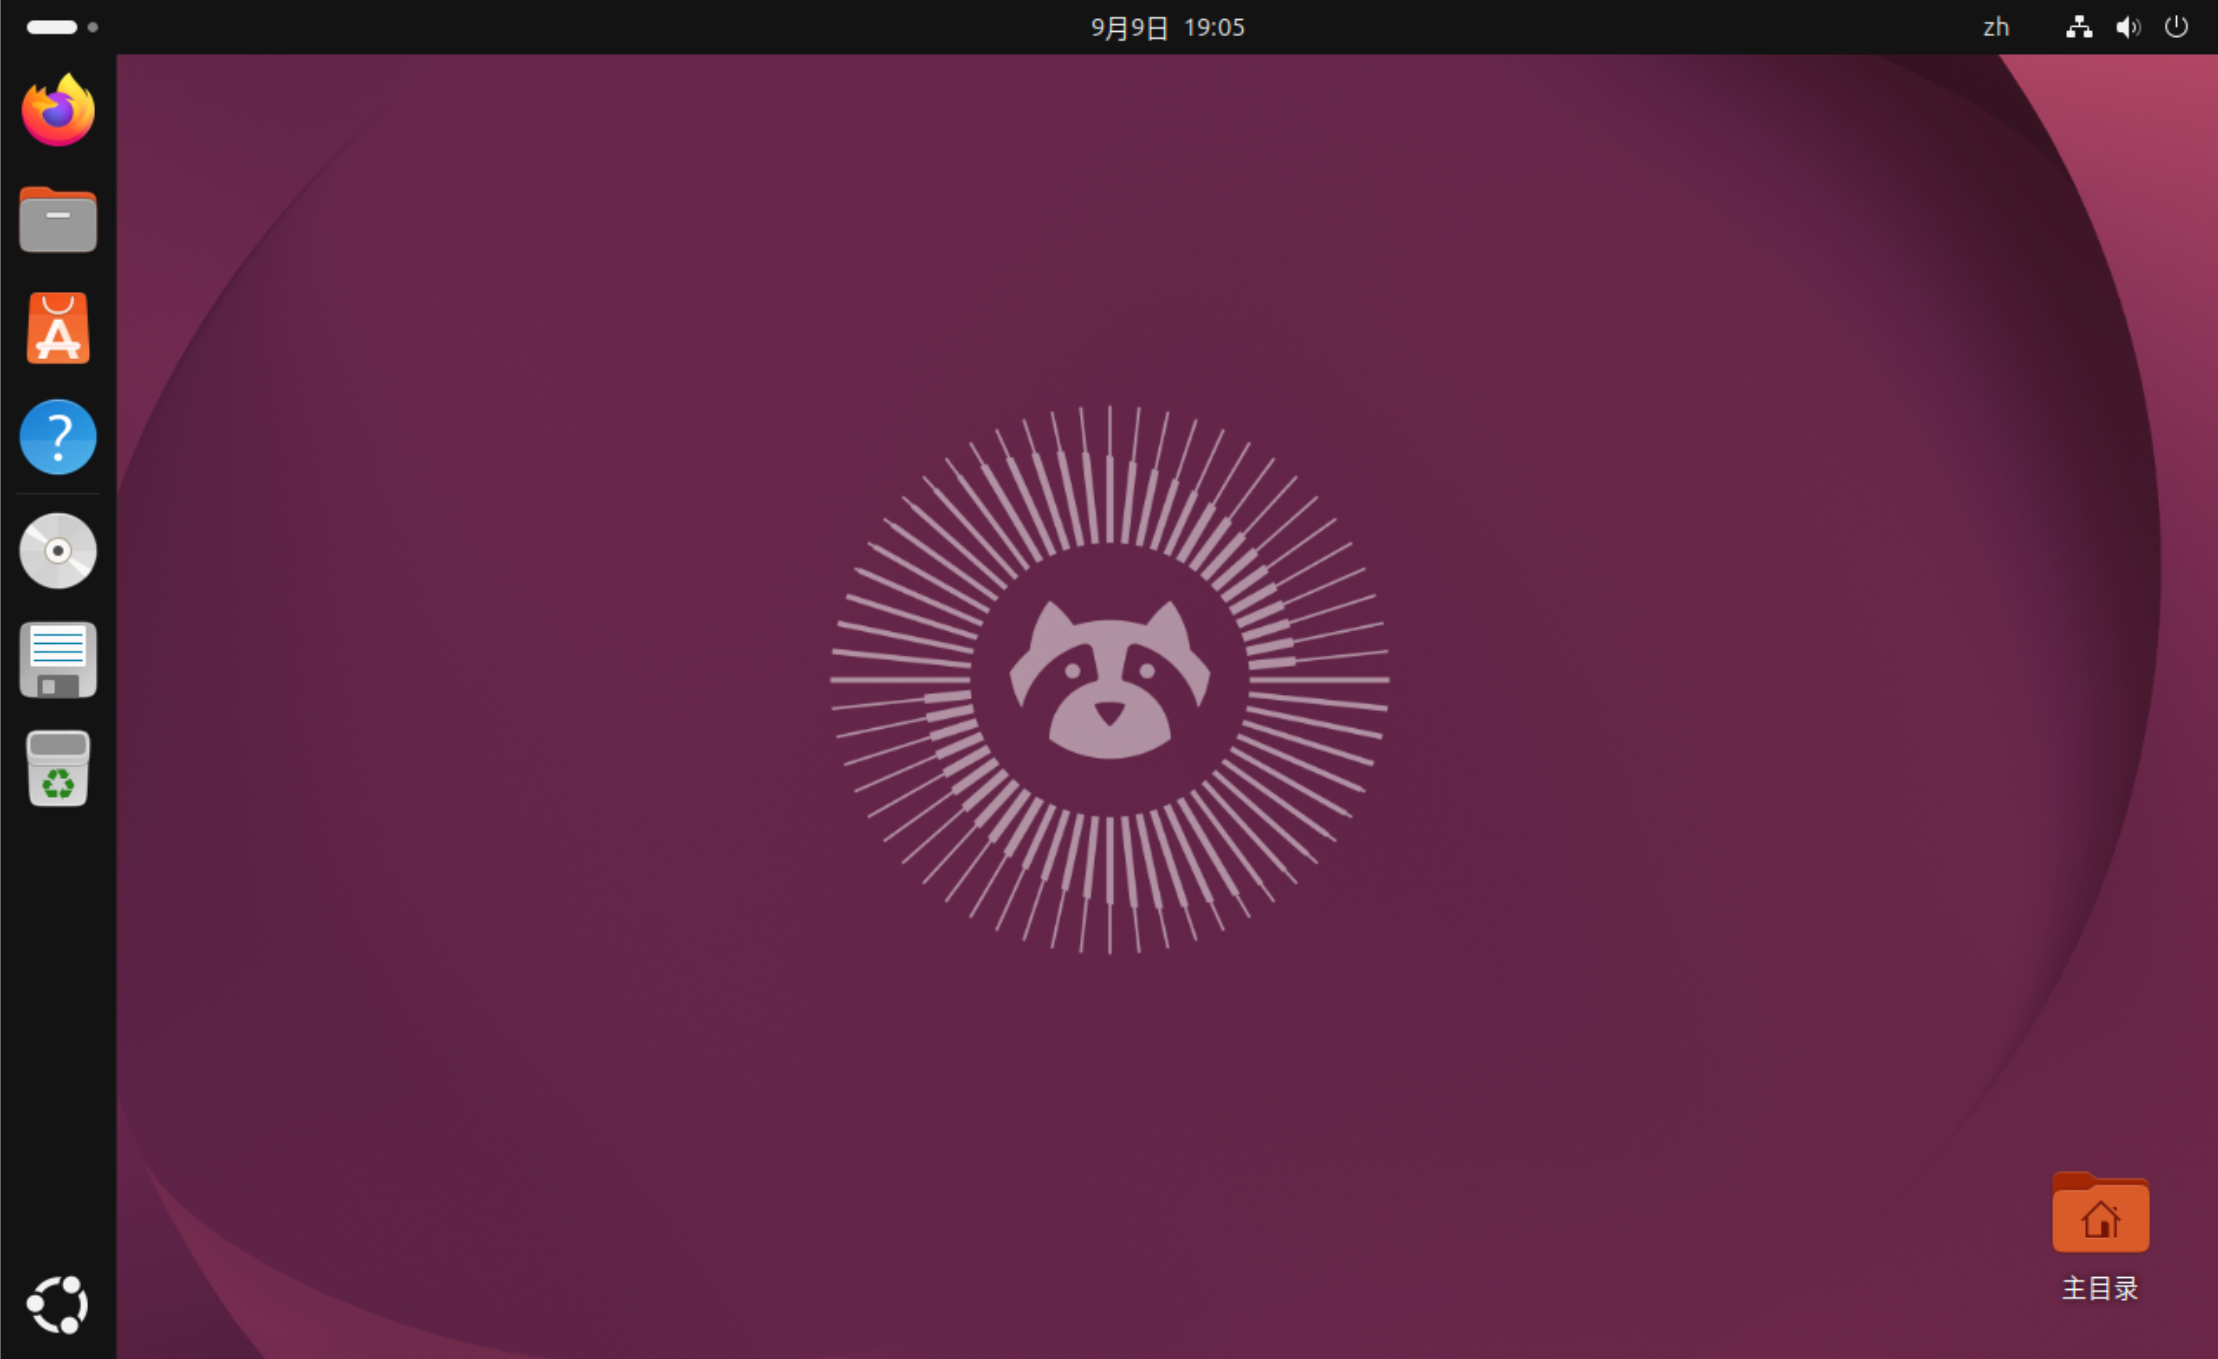
\includegraphics[width=0.8\textwidth]{Figure/Unbuntu界面.png}
  \caption{Ubuntu 桌面界面}
  \label{fig:ubuntu-desktop}
\end{figure}

\subsection{在 VMware 中安装 Ubuntu 虚拟机}

本书的最终目标，是让 ROS 2 在一套 Ubuntu 环境里跑起来。多数读者日常使用的电脑装的是 Windows，直接改装系统代价太大，因此更稳妥的起步方式是：在 Windows 里用虚拟机软件，\emph{模拟出一台完整的 Ubuntu 电脑}。虚拟机可以理解为一台由软件模拟出来的电脑，它有自己的硬盘（磁盘文件）、内存和网卡，Ubuntu 就安装在这台虚拟电脑里。这样做的好处很实在：

\begin{itemize}
    \item \textbf{不影响现有系统}。Ubuntu 只活在虚拟机窗口里，Windows 照常使用；
    \item \textbf{出错可还原}。随时可以拍摄快照，系统被折腾坏了，一键就能恢复到快照时的干净状态；
    \item \textbf{门槛低}。不用重新分区，也不涉及双系统引导，跟着下面的步骤走即可。
\end{itemize}

本小节以 VMware Workstation 为例（该软件现已对个人用户免费）。硬件上建议宿主机内存至少 8 GB，并预留 60 GB 以上的磁盘空间。

\subsubsection{准备安装材料}

需要准备两样东西：Ubuntu 系统镜像，以及 VMware Workstation 软件本身。

Ubuntu 镜像推荐使用 LTS 桌面版。官方下载地址是 \url{https://ubuntu.com/download/desktop}，如果下载速度不理想，清华（TUNA）、阿里云等国内镜像站都有完整镜像，在镜像站里找到 \url{ubuntu-releases} 目录即可。镜像文件名形如 \url{ubuntu-22.04-desktop-amd64.iso}，务必选择 \textbf{desktop}（桌面版），而不是 server（服务器版）；本书后续示例以 22.04 或 24.04 的 LTS 版本为前提。

VMware Workstation 在官网注册下载后即可免费用于个人用途，在 Windows 上按提示安装完成。

\subsubsection{在 VMware 中创建虚拟机}

打开 VMware Workstation，按照下面的步骤创建一台空白虚拟机（先不安装系统）：

\begin{enumerate}
    \item 点击主界面的\textbf{新建虚拟机}，类型选择「典型（推荐）」；
    \item 安装来源选择「\textbf{稍后安装操作系统}」。这里不要直接指定 ISO 文件，否则 VMware 会启用自动安装，反而看不到正常的安装过程；
    \item 客户机操作系统选择 \textbf{Linux}，版本选择 \textbf{Ubuntu 64 位}；
    \item 给虚拟机命名并选择存放位置；
    \item 磁盘容量建议 60 GB 以上，并选择「将虚拟磁盘拆分成多个文件」，这样日后移动、备份虚拟机都很方便；
    \item 点击「自定义硬件」：内存建议 4 GB 以上（最好 8 GB），处理器 2 核以上，网络适配器保持默认的 \textbf{NAT} 即可；
    \item 创建完成后，在左侧选中该虚拟机，打开菜单栏「虚拟机」下的「设置」，在 \textbf{CD/DVD (SATA)} 一栏勾选「启动时连接」，并浏览选择刚才下载的 Ubuntu 镜像文件，确定保存。
\end{enumerate}

\subsubsection{安装 Ubuntu 系统}

点击「开启此虚拟机」，之后的操作都发生在虚拟机窗口里：

\begin{enumerate}
    \item 从镜像引导后，在左侧语言列表选择中文（简体），点击「安装 Ubuntu」；
    \item 键盘布局保持默认即可；
    \item 在「更新和其他软件」界面，建议取消勾选「安装时下载更新」，省去漫长的等待（之后换好国内软件源再更新会快得多）；
    \item 安装类型选择「\textbf{清除整个磁盘并安装 Ubuntu}」。这一步在真实电脑上必须万分谨慎，但在虚拟机里磁盘是虚拟的，可以放心操作；
    \item 确认提示后点击「现在安装」，再点击「继续」；
    \item 时区选择 \textbf{Shanghai}，随后设置用户名和密码。\emph{请务必牢记这个密码}，之后执行 \texttt{sudo} 命令都要用到它；
    \item 等待安装完成。若屏幕提示移除安装介质后按回车，先在 VMware 菜单「虚拟机」下的「设置」里，取消 \textbf{CD/DVD (SATA)} 的「已连接」勾选，再回到虚拟机窗口按回车重启；
    \item 重启后输入密码进入桌面，Ubuntu 虚拟机就装好了。
\end{enumerate}

装好系统后先别急着开始，建议顺手完成三件事，后面能省下不少麻烦：

\begin{itemize}
    \item 安装 VMware Tools，让虚拟机与宿主机顺畅协作（见下一小节）；
    \item 更换软件源为国内镜像：打开「软件和更新」，把「下载自」的服务器改为清华或阿里镜像，之后用 \texttt{apt} 安装软件会快很多；
    \item 拍摄一张快照：在 VMware 菜单「虚拟机」下的「快照」中选择「拍摄快照」。之后系统配置坏了，随时可以恢复到当前这个干净状态。
\end{itemize}

\subsection{VMware Tools 的安装}

VMware Tools 是 VMware 提供的一组驱动和工具，装好之后虚拟机才能和宿主机顺畅协作：窗口大小自动适配分辨率、鼠标在虚拟机内外自由进出、文字可以跨系统复制粘贴、文件可以直接拖拽。过去需要在虚拟机里手动运行官方的闭源安装包，而新版 Ubuntu 完全不必如此：直接用开源的 \texttt{open-vm-tools} 即可。它由 VMware 官方推荐、随系统软件源分发，安装简单、兼容性好，还会随内核自动更新。

\subsubsection{标准安装（推荐）}

以下步骤适用于 Ubuntu 18.04 及以上版本（含 22.04、24.04）。先打开终端，更新软件包列表：

\begin{lstlisting}[language=bash,title={更新软件包列表}]
    sudo apt update
\end{lstlisting}

然后安装核心组件和桌面集成包。桌面版 Ubuntu 需要同时安装 \texttt{open-vm-tools-}\allowbreak\texttt{desktop}，它负责实现分辨率自适应、文件拖拽、复制粘贴等功能：

\begin{lstlisting}[language=bash,title={安装 open-vm-tools 及桌面集成包}]
    sudo apt install open-vm-tools open-vm-tools-desktop -y
\end{lstlisting}

安装完成后重启虚拟机，让服务生效：

\begin{lstlisting}[language=bash,title={重启虚拟机}]
    sudo reboot
\end{lstlisting}

重启回到桌面后，测试宿主机与虚拟机之间的文件拖拽、文字复制粘贴是否正常。如果一切顺利，之后在 Windows 与 Ubuntu 之间交换文件、复制命令就会非常顺手。

\subsubsection{安装失败或残留旧版时的修复}

如果之前手动安装过官方的 VMware Tools，或安装过程报错，可以先卸载清理，再重新安装：

\begin{lstlisting}[language=bash,title={卸载原有组件并清理}]
    sudo apt autoremove open-vm-tools -y
\end{lstlisting}

\begin{lstlisting}[language=bash,title={重新安装}]
    sudo apt install open-vm-tools open-vm-tools-desktop -y
\end{lstlisting}

\begin{lstlisting}[language=bash,title={重启生效}]
    sudo reboot
\end{lstlisting}

\subsubsection{传统手动安装官方 VMware Tools（不推荐）}

仅在 \texttt{open-vm-tools} 无法满足需求时，才考虑手动安装。需要说明的是，手动安装的官方工具与 \texttt{open-vm-tools} 会互相冲突，两者只能选其一；而且每次升级 Linux 内核后，官方闭源版往往需要重新安装一遍，维护成本高，所以本书不推荐这条路线。

确实需要手动安装时，步骤如下。先在 VMware 菜单栏选择「虚拟机」菜单下的「安装 VMware Tools」，虚拟机会自动挂载一个 ISO 镜像。然后进入挂载目录，把安装包拷贝到临时目录并解压：

\begin{lstlisting}[language=bash,title={拷贝安装包并解压}]
    cd /media/$USER/VMware\ Tools
    cp VMwareTools-*.tar.gz /tmp/
    cd /tmp
    tar -zxvf VMwareTools-*.tar.gz
\end{lstlisting}

接着执行安装脚本：

\begin{lstlisting}[language=bash,title={运行安装脚本}]
    cd vmware-tools-distrib
    sudo ./vmware-install.pl
\end{lstlisting}

安装过程中一路按回车接受默认配置即可，完成后重启虚拟机生效。

\section{ROS 是什么}

\subsection{ROS 不是操作系统}

ROS 的全称是 Robot Operating System，中文常译作``机器人操作系统''。这个叫法很有迷惑性：\emph{ROS 并不是一个操作系统}，它不能独立安装在裸机上，而是运行在操作系统（通常是 Ubuntu）之上的一套\emph{开源机器人软件开发框架}。ROS本身并不是一个操作系统，而是可以安装在现在已有的操作系统上（Linux、Windows、Mac）上的 软件库和工具集 。

为什么机器人软件需要这样一套框架？因为一个稍微像样的机器人程序，往往由很多独立的部分组成：读取激光雷达和相机数据、处理感知、做运动规划、控制电机、与人交互……如果每个模块都自己写一套和别人通信的办法，整个系统会迅速变成一团乱麻。ROS 要解决的正是这个问题：它规定了一套统一的通信机制，并提供了大量现成的工具和功能包，让开发者可以专心写自己的那一部分，其余交给生态。

\subsection{核心概念：节点与通信}

ROS 里有两个必须最先建立印象的概念：

\begin{itemize}
    \item \textbf{节点（node）}：一个可以独立运行的程序模块。整个机器人系统可以看作许多节点协作组成的 ``网络''。
    \item \textbf{通信方式}：节点之间通过\emph{话题（topic）}、\emph{服务（service）}、\emph{动作（action）}等方式交换\emph{消息（message）}，消息就是节点间传递的数据包。
\end{itemize}

打个比方：传感器节点像是不断播报路况的广播电台（话题），导航节点像是收听广播的司机；而当你需要打车时那种``一问一答''的交互（服务），又和广播完全不同。这套通信机制的细节会在后面的章节展开，这里先记住``节点 + 通信''这个总框架即可。

\subsection{从 ROS 1 到 ROS 2}

ROS 起源于 2007 年斯坦福大学的一个机器人项目，随后由 Willow Garage 公司推动，逐渐发展成全球机器人研究界的事实标准，积累了庞大的生态。不过随着机器人应用走向工业化和复杂化，ROS 1 的一些先天设计问题开始暴露：

\begin{itemize}
    \item 通信依赖一个中心节点 \texttt{roscore}，它一旦宕机，整个系统就瘫痪；
    \item 以单机为主，多机分布式和实时性支持不足；
    \item 几乎没有安全机制，难以满足工业级要求。
\end{itemize}

于是社区从 2014 年前后开始重新设计，2017 年发布了 ROS 2 的第一个正式发行版。ROS 2 不是 ROS 1 的小修小补，而是一次架构级的重写。今天，ROS 1 已经停止维护（最后一个发行版是 2020 年的 Noetic），新项目都应当基于 ROS 2。本书讲的也是 ROS 2。

\section{ROS 1 与 ROS 2 的主要区别}

把上面的要点归纳成一张对比表，方便查阅：

\begin{center}
\begin{tabular}{|l|l|l|}
\hline
\textbf{对比项} & \textbf{ROS 1} & \textbf{ROS 2} \\
\hline
通信机制 & 自研 TCPROS/UDPROS & 基于 DDS 标准 \\
中心节点 & 依赖 \texttt{roscore} & 去中心化，无需主节点 \\
实时性 & 不支持 & 可通过 DDS 配置支持 \\
多机分布式 & 支持较弱 & 原生良好支持 \\
安全机制 & 几乎没有 & 内置（如 SROS2） \\
支持平台 & 主要 Linux & Linux/Windows/macOS 等 \\
\hline
\end{tabular}
\end{center}

对学习者而言，这些区别并不需要现在就全部弄懂。你只需要记住一个大方向：\emph{学 ROS 2}。后面章节里出现的所有命令和示例，都默认运行在 ROS 2 之上。

\section{ROS 2 与 Ubuntu 版本的搭配}

ROS 2 和 Ubuntu 一样，也有发行版的概念，而且两者高度绑定：官方每两年发布一个 ROS 2 的 LTS 版本，与当年度 Ubuntu 的 LTS 版本一一对应。最常用的组合如下：

\begin{center}
\begin{tabular}{|l|l|l|}
\hline
\textbf{Ubuntu 版本} & \textbf{ROS 2 发行版} & \textbf{说明} \\
\hline
20.04（2020 LTS） & Foxy（2020 LTS） & 较旧，资料丰富 \\
22.04（2022 LTS） & Humble（2022 LTS） & 目前最主流，教程最多 \\
24.04（2024 LTS） & Jazzy（2024 LTS） & 最新，适合新硬件 \\
\hline
\end{tabular}
\end{center}

给初学者的建议很明确：\emph{Ubuntu 22.04 + ROS 2 Humble} 是目前资料最全、社区最活跃、兼容性问题最少的组合，本书的示例也默认基于它。如果你的电脑比较新，安装 22.04 时遇到显卡或硬件驱动问题，再考虑 Ubuntu 24.04 + Jazzy 也不迟。

这里有一条最重要的原则：\emph{不要混搭}。比如在 Ubuntu 20.04 上硬装 Humble，或在 22.04 上装 Foxy，往往会遇到一堆莫名其妙的编译错误，而问题根源只是版本不对。版本搭配对了，后面能少走一半弯路。等你在第二章学会打开终端之后，可以用 \texttt{lsb\_release -a} 这条命令随时查看自己系统的 Ubuntu 版本。

\section{本书的学习路线}

这一章建立的是``地图''，接下来的章节才是``走路''：

\begin{itemize}
    \item \textbf{第二章} Ubuntu 常用指令：学会打开终端，掌握文件、目录、权限等最常用的命令，这是之后所有操作的地基；
    \item 之后是安装与配置 ROS 2，亲手把环境跑起来；
    \item 再往后深入节点、话题、服务等核心概念，配合小例子逐个验证；
    \item 最后把各部分串起来，完成小型机器人程序，体会完整的工作流。
\end{itemize}

如果你现在对 ``Ubuntu 到底是什么、ROS 能干什么'' 已经有了大致印象，那这一章的任务就完成了。翻开第二章，我们从打开终端开始。

% ============ 文件结尾 ============
% 整书模式(被 main.tex 引用): 读到这里即 \endinput 交还控制权,
% 不会执行下方的 \end{document}。
\ifcsname wholebook\endcsname
\expandafter\endinput
\fi

% 单独编译模式: 在顶层(无未闭合条件)执行 \end{document} 收尾。
\end{document}

% ============================================================
% 第 2 章 Ubuntu 常用指令
% ============================================================
% 魔术注释(供编辑器识别编译方式):
% !TEX program = xelatex
% !TEX encoding = UTF-8
% ============================================================
% 本文件有两种编译方式:
%   方式一(单独编译本章): 直接用 XeLaTeX 编译本文件, 只输出本章内容。
%   方式二(编译整本书):   编译 main.tex, 本文件会被自动 \input 引入。
% 两种方式都共用 preamble.tex, 请保持本文件与 main.tex、
% preamble.tex 位于同一目录。
% 注意: 单独编译时章编号从第 1 章重新计起, 不影响整书编号。
% ============================================================
% 单独编译开关:
%   被 main.tex 引用时, main.tex 已定义 \wholebook, 于是跳过
%   \documentclass 与导言区, 只写正文; 直接编译本文件时,
%   \wholebook 未定义, 就自动补上完整的文档头。
\ifcsname wholebook\endcsname
\else
\documentclass[12pt,a4paper]{ctexbook}
% ============================================================
% 共享导言区 preamble.tex
% 本文件被 main.tex(整书编译)和各章文件(单独编译)共同引用,
% 从而保证两种编译方式下的宏包与样式完全一致。
% 注意: 本文件不含 \documentclass, 只放宏包与样式设置。
% ============================================================
\usepackage[a4paper,margin=1.1in]{geometry}
\usepackage{graphicx}
\usepackage{listings}
\usepackage{xcolor}
\usepackage[hidelinks]{hyperref}
\usepackage{tikz}
\usetikzlibrary{positioning,arrows.meta,decorations.pathreplacing,calc}
\usepackage{booktabs}

% 代码环境样式设置
\lstset{
    basicstyle=\ttfamily\small,
    keywordstyle=\color{blue}\ttfamily,
    commentstyle=\color{gray}\ttfamily,
    stringstyle=\color{red}\ttfamily,
    backgroundcolor=\color{gray!8},
    frame=single,
    rulecolor=\color{gray!40},
    breaklines=true,
    showstringspaces=false,
    columns=fullflexible,
    keepspaces=true,
    % 允许中文注释/内容正常显示
    extendedchars=true,
    literate={
        {·}{{\cdot}}1
    }
}

\begin{document}
\fi

\chapter{Ubuntu 常用指令}
\section{打开终端}
第一件事是学会打开终端。常用的终端打开方式无外乎两种：
\begin{itemize}
    \item 使用快捷键 Ctrl+Alt+T
    \item 文件夹中右击打开 \textit{open in Terminal}
\end{itemize}
\section{Linux中的常用命令}
\subsection{ls命令}
就是 list 的缩写，通过 ls 命令不仅可以查看 \textit{linux} 文件夹包含的文件，而且可以查看文件权限(包括目录、文件夹、文件权限)，查看目录信息等等。
\begin{lstlisting}[language=bash,title={ls 命令常用参数}]
ls -a  列出目录所有文件，包含以.开始的隐藏文件
ls -A  列出除.及..的其它文件
ls -r  反序排列
ls -t  以文件修改时间排序
ls -S  以文件大小排序
ls -h  以易读大小显示
ls -l  列出文件的权限、所有者、文件大小等详细信息
\end{lstlisting}
实例：
\begin{lstlisting}[language=bash,title={按易读方式按时间反序排序，并显示文件详细信息}]
    ls -lhrt
\end{lstlisting}

\begin{lstlisting}[language=bash,title={按大小反序显示文件详细信息}]
    ls -lrS
\end{lstlisting}
\begin{lstlisting}[language=bash,title={列出当前目录中所有以"t"开头的目录的详细内容}]
    ls -l t*
\end{lstlisting}
\begin{lstlisting}[language=bash,title={列出文件绝对路径（不包含隐藏文件）}]
    ls | sed "s:^:`pwd`/:"
\end{lstlisting}
\begin{lstlisting}[language=bash,title={列出文件绝对路径（包含隐藏文件）}]
    find $pwd -maxdepth 1 | xargs ls -ld
\end{lstlisting}
\begin{figure}[h]
  \centering
  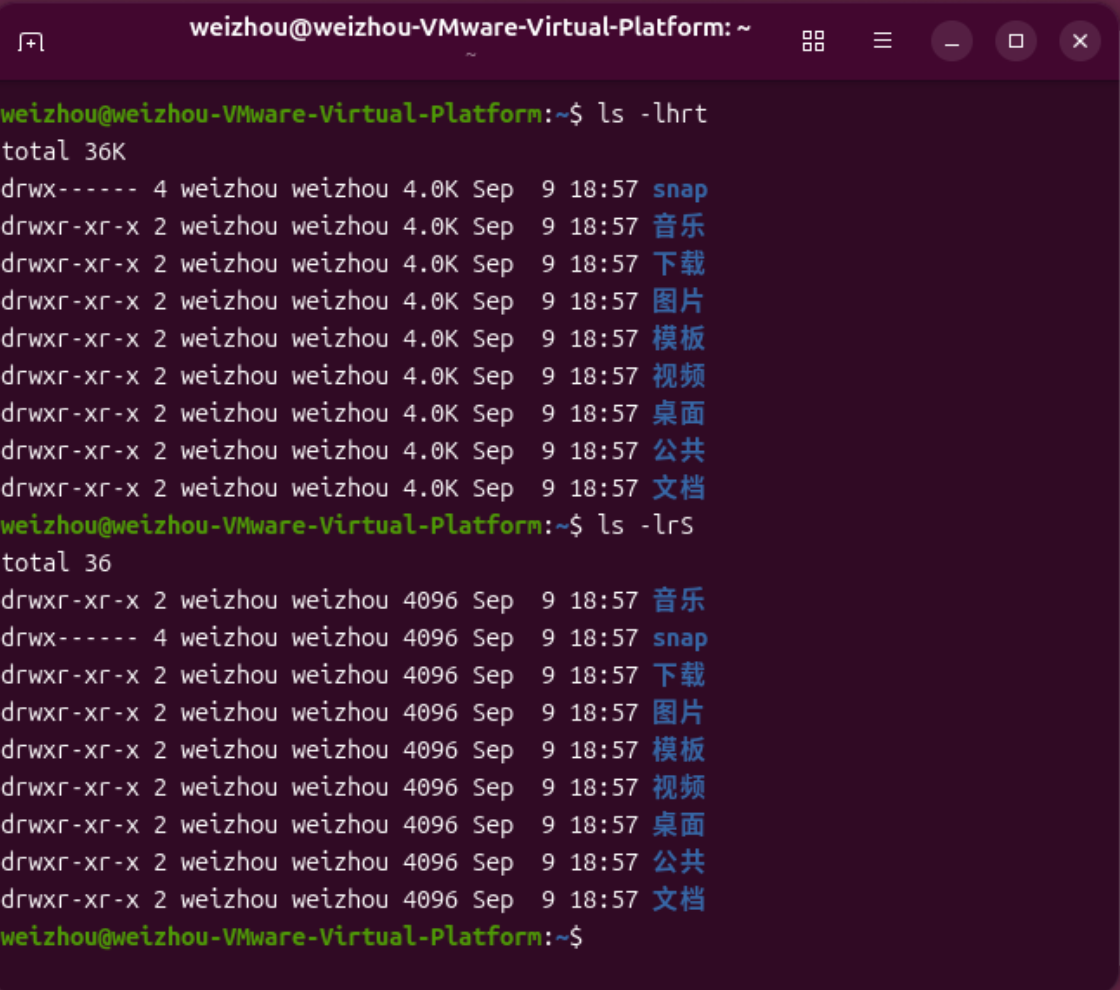
\includegraphics[width=0.8\textwidth]{Figure/ls命令示例}
  \caption{ls命令示例}
  \label{fig:ls命令示例}
\end{figure}

\subsection{cd 命令}
cd(changeDirectory) 命令语法：
\begin{lstlisting}[language=bash,title={cd(changeDirectory) 命令语法：}]
    cd [目录名]
\end{lstlisting}
说明：切换当前目录至 dirName。

示例：
\begin{lstlisting}[language=bash,title={进入要目录}]
    cd /
\end{lstlisting}
\begin{lstlisting}[language=bash,title={进入 "home" 目录}]
    cd ~
\end{lstlisting}
\begin{lstlisting}[language=bash,title={进入上一次工作路径}]
    cd -
\end{lstlisting}
\begin{lstlisting}[language=bash,title={把上个命令的参数作为cd参数使用。}]
    cd !$
\end{lstlisting}

\begin{figure}[h]
  \centering
  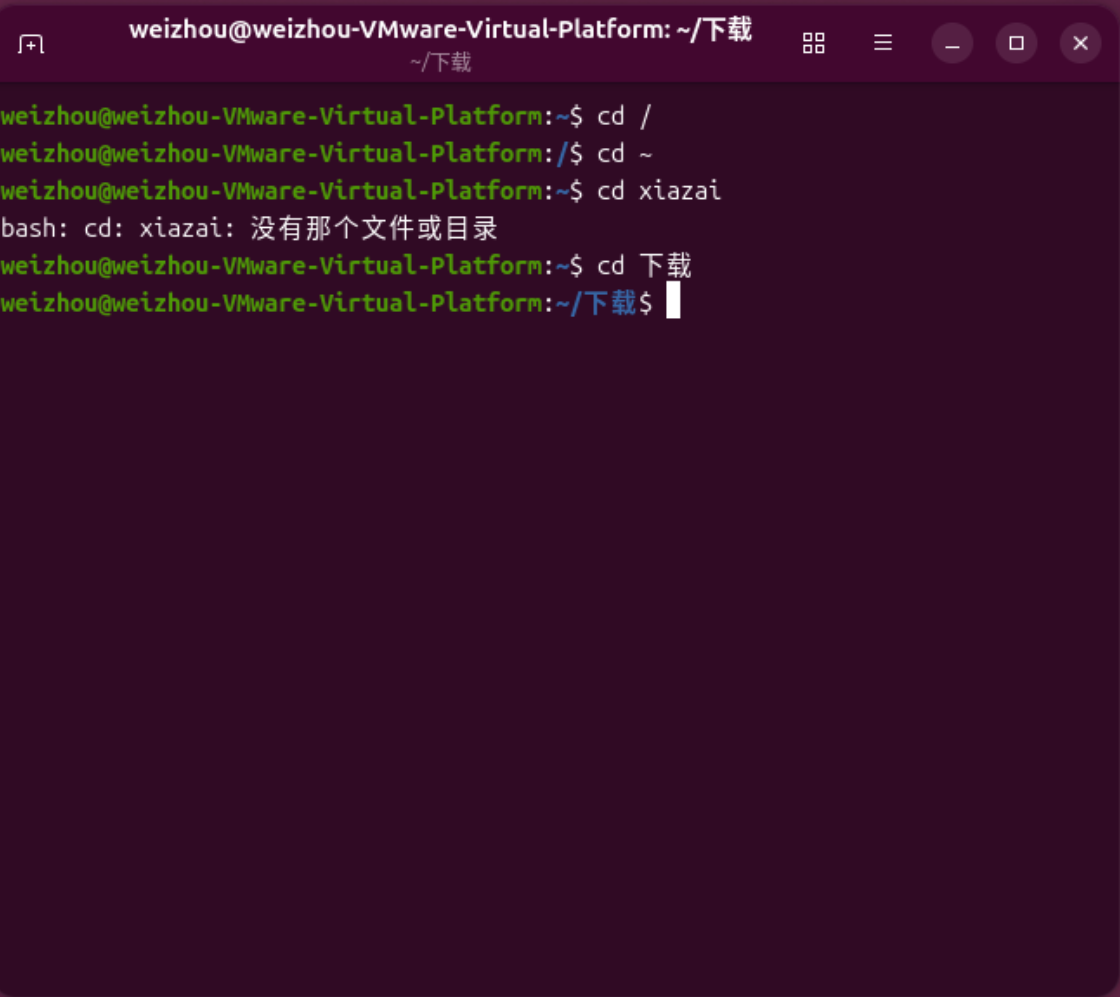
\includegraphics[width=0.8\textwidth]{Figure/cd命令示例}
  \caption{cd命令示例}
  \label{fig:cd命令示例}
\end{figure}

\subsection{pwd 命令}
pwd 命令用于查看当前工作目录路径。它是初学者最常用来确认``我现在在哪''的命令。
\begin{lstlisting}[language=bash,title={查看当前路径}]
    pwd
\end{lstlisting}
\begin{lstlisting}[language=bash,title={查看软链接的实际路径}]
    pwd -P
\end{lstlisting}
\begin{figure}[h]
  \centering
  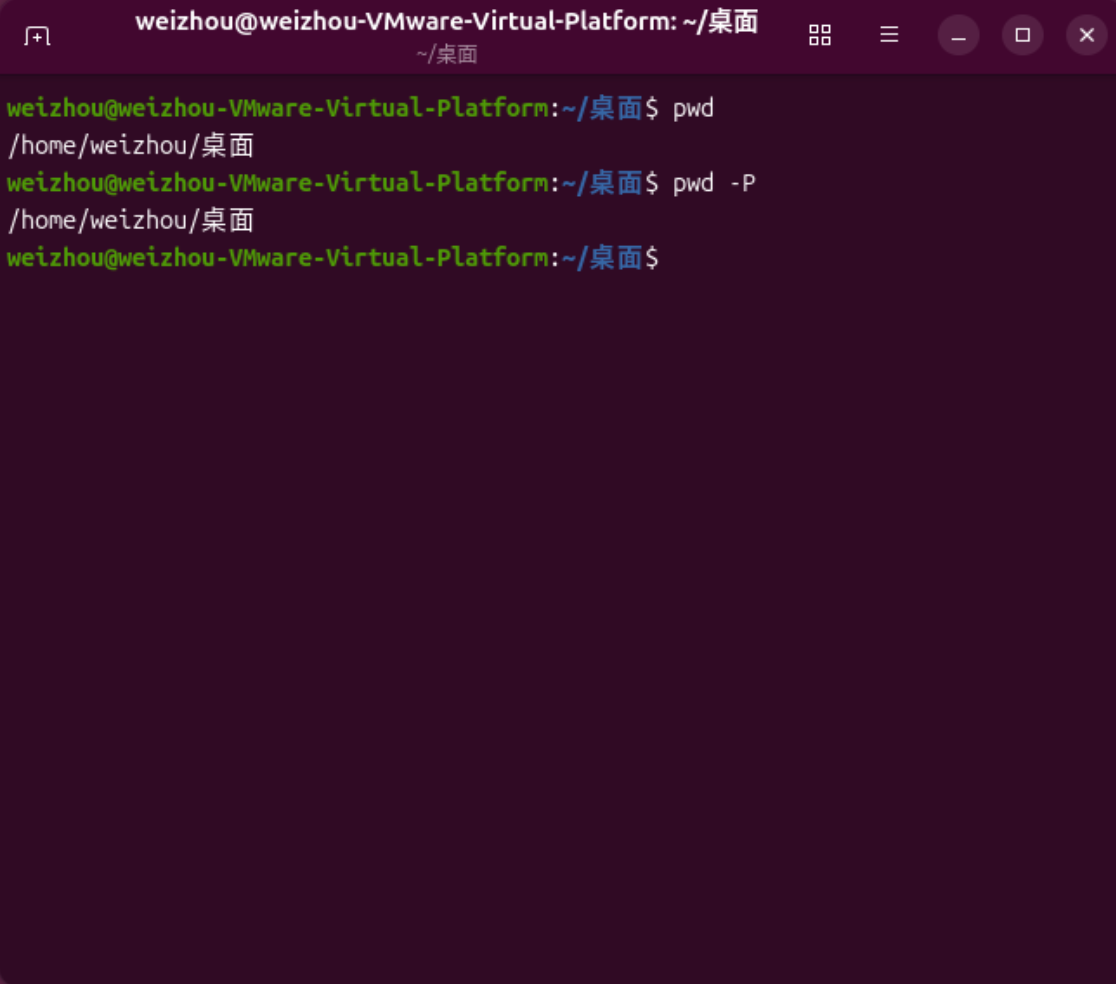
\includegraphics[width=0.8\textwidth]{Figure/pwd命令示例}
  \caption{pwd命令示例}
  \label{fig:pwd命令示例}
\end{figure}

\subsection{mkdir 命令}
mkdir 命令用于创建文件夹。
\begin{lstlisting}[language=bash,title={mkdir 常用参数}]
mkdir -m    对新建目录设置存取权限
mkdir -p    若路径中某些目录尚不存在, 系统会自动建立(一次建多级)
\end{lstlisting}
实例：
\begin{lstlisting}[language=bash,title={当前工作目录下创建名为 t 的文件夹}]
    mkdir t
\end{lstlisting}
\begin{lstlisting}[language=bash,title={在 tmp 下创建 path test/t1/t, 若目录不存在则一并建立}]
    mkdir -p /tmp/test/t1/t
\end{lstlisting}

\subsection{rm 命令}
删除一个或多个文件或目录。如果不加 \textit{-r} 选项，rm 不会删除目录。删除文件通常仍可以恢复，但删除目录需谨慎。
\begin{lstlisting}[language=bash,title={rm 常用参数}]
rm -i    删除前逐一询问确认
rm -r    递归删除(连同子目录一起删除)
rm -f    强制删除, 不提示
\end{lstlisting}
实例：
\begin{lstlisting}[language=bash,title={删除任何 .log 文件, 删除前逐一询问}]
    rm -i *.log
\end{lstlisting}
\begin{lstlisting}[language=bash,title={删除 test 子目录及其中所有内容, 不一一确认}]
    rm -rf test
\end{lstlisting}
\begin{lstlisting}[language=bash,title={删除以 - 开头的文件(用 -- 结束选项) }]
    rm -- -f*
\end{lstlisting}

\subsection{cp 命令}
将源文件复制到目标文件，或将多个源文件复制到目标目录。
\begin{lstlisting}[language=bash,title={cp 常用参数}]
cp -i    目标文件已存在时提示是否覆盖
cp -r    复制目录及目录内所有内容
cp -a    保持原文件的时间等属性
cp -s    建立符号链接(快捷方式)
\end{lstlisting}
实例：
\begin{lstlisting}[language=bash,title={复制 a.txt 到 test 目录, 保持时间, 存在则提示}]
    cp -ai a.txt test
\end{lstlisting}
\begin{lstlisting}[language=bash,title={为 a.txt 建立一个链接(快捷方式)}]
    cp -s a.txt link_a.txt
\end{lstlisting}

\subsection{mv 命令}
移动文件，或修改文件／目录名。当第二个参数是目录时，将第一个参数（可以是多个）移动到该目录。
\begin{lstlisting}[language=bash,title={mv 常用参数}]
mv -i    目标已存在时提示是否覆盖
\end{lstlisting}
实例：
\begin{lstlisting}[language=bash,title={将文件 test.log 改名为 test1.txt}]
    mv test.log test1.txt
\end{lstlisting}
\begin{lstlisting}[language=bash,title={把多个文件移动到根的 test3 目录}]
    mv log1.txt log2.txt log3.txt /test3
\end{lstlisting}
\begin{lstlisting}[language=bash,title={移动当前目录下所有文件到上一级目录}]
    mv * ../
\end{lstlisting}

\subsection{cat 命令}
cat 主要有三大功能：一次显示整个文件；从键盘创建一个新文件；将几个文件合并成一个文件。
\begin{lstlisting}[language=bash,title={cat 常用参数}]
cat -b    对非空输出行号
cat -n    输出所有行号
\end{lstlisting}
实例：
\begin{lstlisting}[language=bash,title={一次显示整个文件}]
    cat filename
\end{lstlisting}
\begin{lstlisting}[language=bash,title={从键盘创建一个文件(只能新建, 不能编辑已有文件)}]
    cat > filename
\end{lstlisting}
\begin{lstlisting}[language=bash,title={把 log2012.log 内容加上行号后写进 log2013.log}]
    cat -n log2012.log log2013.log
\end{lstlisting}
\begin{lstlisting}[language=bash,title={反向列示文件(与 cat 相反)}]
    tac log.txt
\end{lstlisting}

\subsection{more 命令}
功能类似于 cat，但会一页一页显示，方便逐页阅读。按空格键往下翻一页，按 \textit{b} 键往回翻一页，按 \textit{q} 键退出。
\begin{lstlisting}[language=bash,title={more 常用参数}]
more +n    从第 n 行开始显示
more -n    定义屏幕大小为 n 行
more -s    把连续多个空行显示为一行
\end{lstlisting}
实例：
\begin{lstlisting}[language=bash,title={显示文件中从第 3 行起的内容}]
    more +3 text.txt
\end{lstlisting}
\begin{lstlisting}[language=bash,title={借助管道让 ls -l 每次只显示 5 行}]
    ls -l | more -5
\end{lstlisting}

\subsection{less 命令}
less 与 more 类似，但使用 less 可以随意前后浏览文件，more 只能向前。而且 less 在查看之前不会加载整个文件，更适合大文件。
\begin{lstlisting}[language=bash,title={less 常用操作}]
/字符串    向下搜索字符串
?字符串    向上搜索字符串
n          重复前一个搜索
N          反向重复前一个搜索
空格        滚动一页
b          向后翻一页
-q         退出
\end{lstlisting}
实例：
\begin{lstlisting}[language=bash,title={查看进程信息并通过 less 分页显示(带行号)}]
    ps -aux | less -N
\end{lstlisting}
\begin{lstlisting}[language=bash,title={查看多个文件(按 n 下一个, p 前一个)}]
    less 1.log 2.log
\end{lstlisting}

\subsection{head 命令}
显示文件的开头内容，默认显示前 10 行。
\begin{lstlisting}[language=bash,title={head 常用参数}]
head -n <行数>    显示的行数
head -c <字节数>  显示前多少个字节
\end{lstlisting}
实例：
\begin{lstlisting}[language=bash,title={显示 1.log 文件中前 20 行}]
    head 1.log -n 20
\end{lstlisting}
\begin{lstlisting}[language=bash,title={显示最后 10 行(行数为负数表示从后往前数)}]
    head -n -10 t.log
\end{lstlisting}

\subsection{tail 命令}
显示文件末尾内容，常用来查看日志文件。
\begin{lstlisting}[language=bash,title={tail 常用参数}]
tail -f    循环读取(适合查看动态增加的日志)
tail -n <行数>  显示行数(从后往前)
\end{lstlisting}
实例：
\begin{lstlisting}[language=bash,title={循环读取逐渐增加的文件内容}]
    tail -f ping.log
\end{lstlisting}

\subsection{which、whereis、locate、find 命令}
这四个命令都能用来找文件，但原理和适用场景各不相同：
\begin{itemize}
    \item \textbf{which} 在 PATH 中查找可执行命令的位置，返回第一个匹配结果。
    \item \textbf{whereis} 只搜索程序名相关的二进制、帮助和源码文件，速度快。
    \item \textbf{locate} 基于系统数据库查找文件，速度很快，但新建文件可能找不到。
    \item \textbf{find} 实际遍历硬盘查找文件，最准确但最慢。
\end{itemize}
实例：
\begin{lstlisting}[language=bash,title={查看 ls 命令是否存在及其位置}]
    which ls
\end{lstlisting}
\begin{lstlisting}[language=bash,title={查找 locate 程序的相关文件}]
    whereis locate
\end{lstlisting}
\begin{lstlisting}[language=bash,title={查找与 pwd 相关的所有文件}]
    locate pwd
\end{lstlisting}
\begin{lstlisting}[language=bash,title={在当前目录查找以 .log 结尾的文件}]
    find ./ -name '*.log'
\end{lstlisting}
\begin{lstlisting}[language=bash,title={查找 /opt 目录下权限为 777 的文件}]
    find /opt -perm 777
\end{lstlisting}
\begin{lstlisting}[language=bash,title={查找更改时间在 10 日以前的文件并删除(无提示)}]
    find . -type f -mtime +10 -exec rm -f {} \;
\end{lstlisting}

\subsection{grep 命令}
强大的文本搜索命令，全称 Global Regular Expression Print，即全局正则表达式搜索。它在文件或多个文件中搜索字符串模板，结果输出到标准输出，不改变原文件内容。
\begin{lstlisting}[language=bash,title={grep 常用参数}]
grep -c    计算符合样式的列数
grep -i    忽略大小写
grep -l    只列出文件名
grep -n    显示匹配行所在行号
grep -R    递归查找文件夹
\end{lstlisting}
实例：
\begin{lstlisting}[language=bash,title={查找指定进程}]
    ps -ef | grep svn
\end{lstlisting}
\begin{lstlisting}[language=bash,title={从文件夹递归查找以 grep 开头的行, 只列出文件}]
    grep -lR '^grep' /tmp
\end{lstlisting}
\begin{lstlisting}[language=bash,title={显示包含 ed 或 at 内容的行为}]
    grep -E 'ed|at' test.txt
\end{lstlisting}

\subsection{wc 命令}
wc(word count) 用于统计指定文件中字节数、单词数、行数，并将统计结果输出。
\begin{lstlisting}[language=bash,title={wc 常用参数}]
wc -c    统计字节数
wc -l    统计行数
wc -m    统计字符数
wc -w    统计单词数
\end{lstlisting}
实例：
\begin{lstlisting}[language=bash,title={统计文件的 行数 单词数 字节数}]
    wc text.txt
\end{lstlisting}
\begin{lstlisting}[language=bash,title={统计输出的行数}]
    cat test.txt | wc -l
\end{lstlisting}

\subsection{chmod 命令}
用于改变 Linux 系统文件或目录的访问权限。权限用 r(读)、w(写)、x(执行)表示，对应数字为 4、2、1。每一文件有三组权限：属主、属组、其他用户。
\begin{lstlisting}[language=bash,title={chmod 常用参数}]
chmod -R    递归处理目录及子目录下所有文件
\end{lstlisting}
权限代号：
\begin{lstlisting}[language=bash,title={权限数字对应}]
r = 4    读
w = 2    写
x = 1    执行
\end{lstlisting}
实例：
\begin{lstlisting}[language=bash,title={增加文件 t.log 所有用户的可执行权限}]
    chmod a+x t.log
\end{lstlisting}
\begin{lstlisting}[language=bash,title={属主读写执行(7), 属组读执行(5), 其他执行(1)}]
    chmod 751 t.log
\end{lstlisting}
\begin{lstlisting}[language=bash,title={将 test 目录及子目录所有文件添加可读权限}]
    chmod u+r,g+r,o+r -R text/
\end{lstlisting}

\subsection{tar 命令}
用来打包和解压文件。注意 tar 本身只打包不压缩，压缩与解压是调用其他工具（如 gzip、bzip2）完成的。常用的两招是 \textit{tar zcvf} 打包压缩、\textit{tar zxvf} 解压。
\begin{lstlisting}[language=bash,title={tar 常用参数}]
-c    建立新的压缩文件
-x    从压缩包中解压
-t    显示压缩文件中的内容
-z    支持 gzip 压缩
-j    支持 bzip2 压缩
-v    显示操作过程
-f    指定压缩文件名
\end{lstlisting}
实例：
\begin{lstlisting}[language=bash,title={将文件全部打包成 tar 包}]
    tar -cvf log.tar log1.log log2.log
\end{lstlisting}
\begin{lstlisting}[language=bash,title={将 /etc 下所有文件和目录打包并用 gz 压缩}]
    tar -zcvf /tmp/etc.tar.gz /etc
\end{lstlisting}
\begin{lstlisting}[language=bash,title={查看刚打包的文件内容(必须加 z, 因为用 gzip 压缩)}]
    tar -ztvf /tmp/etc.tar.gz
\end{lstlisting}
\begin{lstlisting}[language=bash,title={解压}]
    tar -zxvf filename.tar.gz
\end{lstlisting}

\subsection{ps 命令}
ps(process status) 用来查看当前运行的进程状态，一次性查看。如需动态连续结果，用 \textit{top}。
\begin{lstlisting}[language=bash,title={ps 常用参数}]
ps -A    显示所有进程
ps -e    显示所有进程(等同 -A)
ps -f    显示进程间的关系(完整格式)
ps -aux  显示所有包含其他信息的进程
\end{lstlisting}
实例：
\begin{lstlisting}[language=bash,title={显示当前所有进程环境变量及进程间关系}]
    ps -ef
\end{lstlisting}
\begin{lstlisting}[language=bash,title={与 grep 联用查找某进程}]
    ps -aux | grep apache
\end{lstlisting}

\subsection{top 命令}
动态显示当前系统正在执行的进程信息，包括进程 ID、CPU 占用率、内存占用率等。交互界面里按 \textit{q} 退出。
\begin{lstlisting}[language=bash,title={top 常用参数}]
top -p <进程号>    指定进程显示
top -n <次数>      循环显示次数
\end{lstlisting}
\begin{lstlisting}[language=bash,title={top 交互命令}]
P    按 CPU 使用率排序
M    按内存使用率排序
q    退出
\end{lstlisting}

\subsection{free 命令}
显示系统内存使用情况，包括物理内存、交换区内存(swap)和内核缓冲区内存。
\begin{lstlisting}[language=bash,title={free 常用参数}]
free -m    以 MB 为单位显示
free -g    以 GB 为单位显示
free -s <秒>  每隔多少秒持续显示
\end{lstlisting}
实例：
\begin{lstlisting}[language=bash,title={显示内存使用情况}]
    free -m
\end{lstlisting}

\subsection{df 命令}
显示磁盘空间使用情况，获取硬盘已占用多少、还剩多少等信息。
\begin{lstlisting}[language=bash,title={df 常用参数}]
df -h    以易读方式显示
df -T    列出文件系统类型
df -a    全部文件系统列表
\end{lstlisting}
实例：
\begin{lstlisting}[language=bash,title={以易读方式列出所有文件系统及其类型}]
    df -haT
\end{lstlisting}

\subsection{du 命令}
查看文件和目录的磁盘使用空间，与 df 不同，du 针对的是具体文件或目录。
\begin{lstlisting}[language=bash,title={du 常用参数}]
du -h    以易读方式显示文件大小
du -s    仅显示总计
du -a    显示目录中所有文件大小
\end{lstlisting}
实例：
\begin{lstlisting}[language=bash,title={以易读方式显示文件夹内及子文件夹大小}]
    du -h scf/
\end{lstlisting}
\begin{lstlisting}[language=bash,title={显示几个文件各自占用空间并统计总和}]
    du -hc test/ scf/
\end{lstlisting}

\subsection{ln 命令}
为文件在另一个位置建立一个链接。软链接(\textit{ln -s})类似于 Windows 里的快捷方式，可跨文件系统、可用于目录；硬链接(\textit{ln})以文件副本形式存在，但同一文件系统内才可创建，且不占用实际空间。无论改哪一处，其余链接都会同步变化。
\begin{lstlisting}[language=bash,title={ln 常用参数}]
ln -s    软链接(符号链接)
ln -v    显示详细处理过程
\end{lstlisting}
实例：
\begin{lstlisting}[language=bash,title={给文件创建软链接并显示操作信息}]
    ln -sv source.log link.log
\end{lstlisting}

\subsection{date 与 cal 命令}
date 显示或设定系统的日期与时间；cal 显示公历（阳历）日历。
\begin{lstlisting}[language=bash,title={date 常用格式}]
%Y    年份(四位数)
%m    月份(01-12)
%d    日期(01-31)
%H    小时(00-23)
%M    分钟(00-59)
\end{lstlisting}
实例：
\begin{lstlisting}[language=bash,title={显示指定日期格式}]
    date +%Y%m%d
\end{lstlisting}
\begin{lstlisting}[language=bash,title={显示下一天}]
    date -d "+1 day" +%Y%m%d
\end{lstlisting}
\begin{lstlisting}[language=bash,title={显示 2013 年每个月的日历}]
    cal -y 2013
\end{lstlisting}
\begin{lstlisting}[language=bash,title={将星期一作为第一列, 显示前中后三月}]
    cal -3m
\end{lstlisting}

\subsection{kill 命令}
发送指定信号给相应进程。默认发送 SIGTERM(15) 终止指定进程，若无法终止可用 \textit{-KILL}（发送 SIGKILL，9）强制结束进程。用 ps 或 jobs 查看进程号；root 用户可影响所有用户的进程，普通用户只能影响自己。
\begin{lstlisting}[language=bash,title={kill 常用参数}]
kill -l           列出全部信号名称
kill -9 <PID>     强制结束进程
\end{lstlisting}
实例：
\begin{lstlisting}[language=bash,title={先查找进程 pro1, 然后强制杀掉}]
    kill -9 $(ps -ef | grep pro1)
\end{lstlisting}

\section{鱼香ROS的指令}
上面的是Linux的常用指令，下面一个指令非常重要，是咱们使用ROS系统可以会的指令，极大节省时间：
\begin{lstlisting}[language=bash,title={一键安装}]
    wget http://fishros.com/install -O fishros && . fishros
\end{lstlisting}
这条指令来自我关注的博主“鱼香ROS”，非常好用。效果如下图：
\begin{figure}[h]
  \centering
  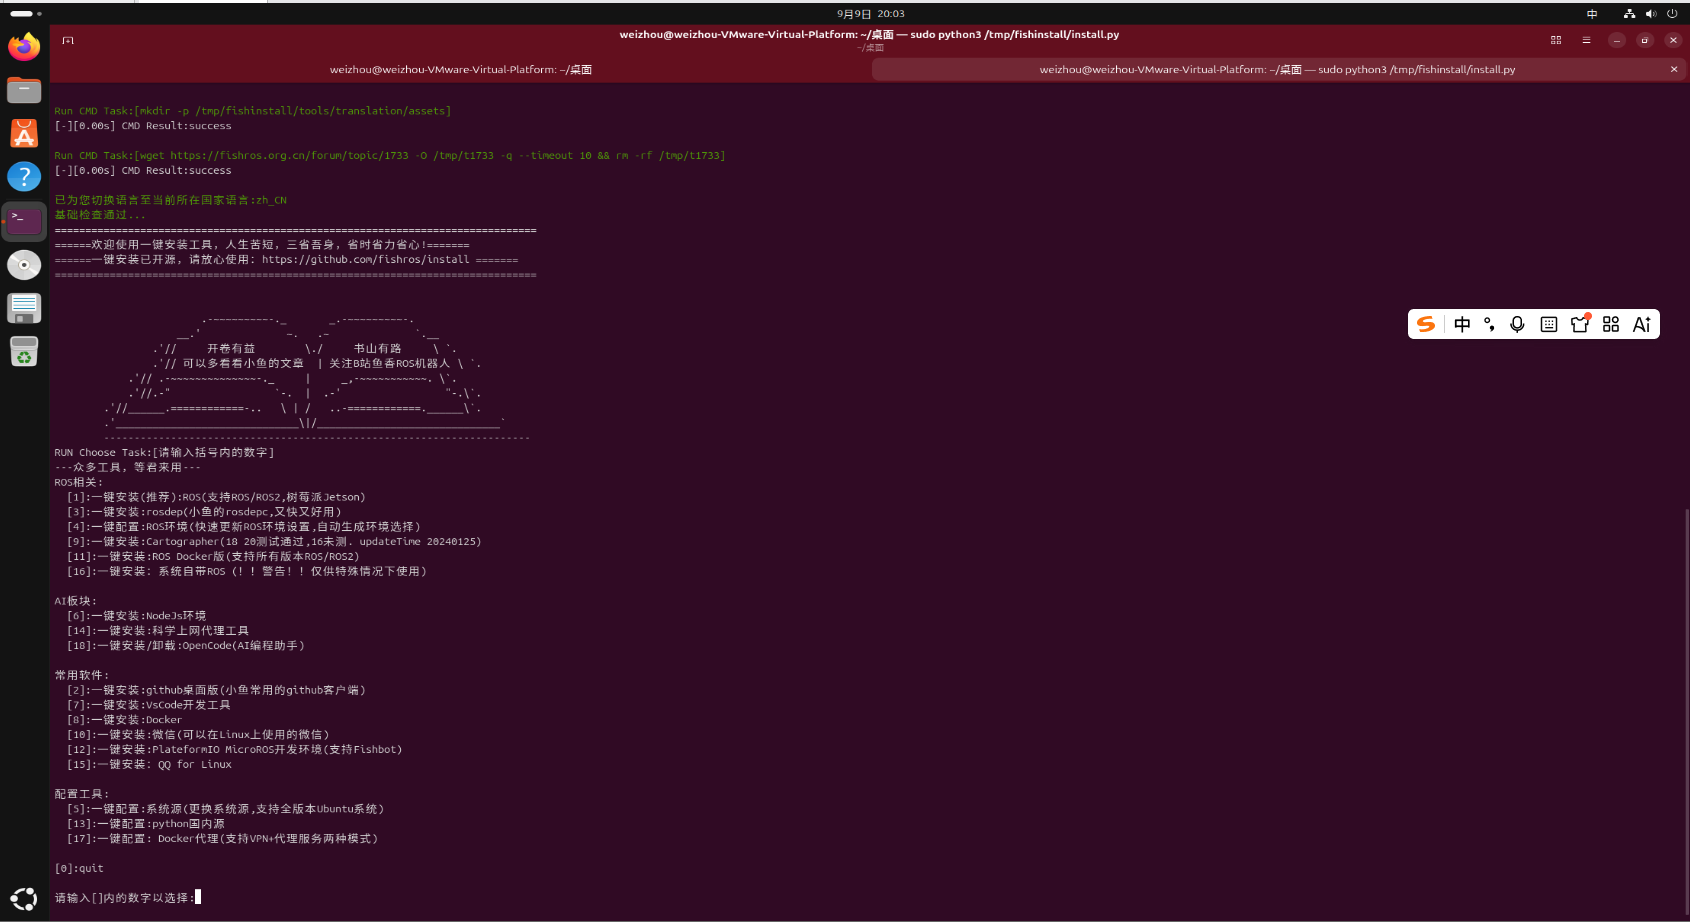
\includegraphics[width=0.6\textwidth]{Figure/小鱼的一键安装命令.png}
  \caption{小鱼的一键安装命令}
  \label{fig:小鱼的一键安装命令}
\end{figure}
显然，包含了咱们要用的几乎所有工具。

\section{用自然语言来使用Unbuntu}
AI时代，古法编程的艺术仍在流传，但Vibe Coding已经成为主流。我选择在保留自己读写代码能力的同时，先装一个npm,再装上opencode，然后美美使用中文使用Unbuntu（doge）
\begin{figure}[h]
  \centering
  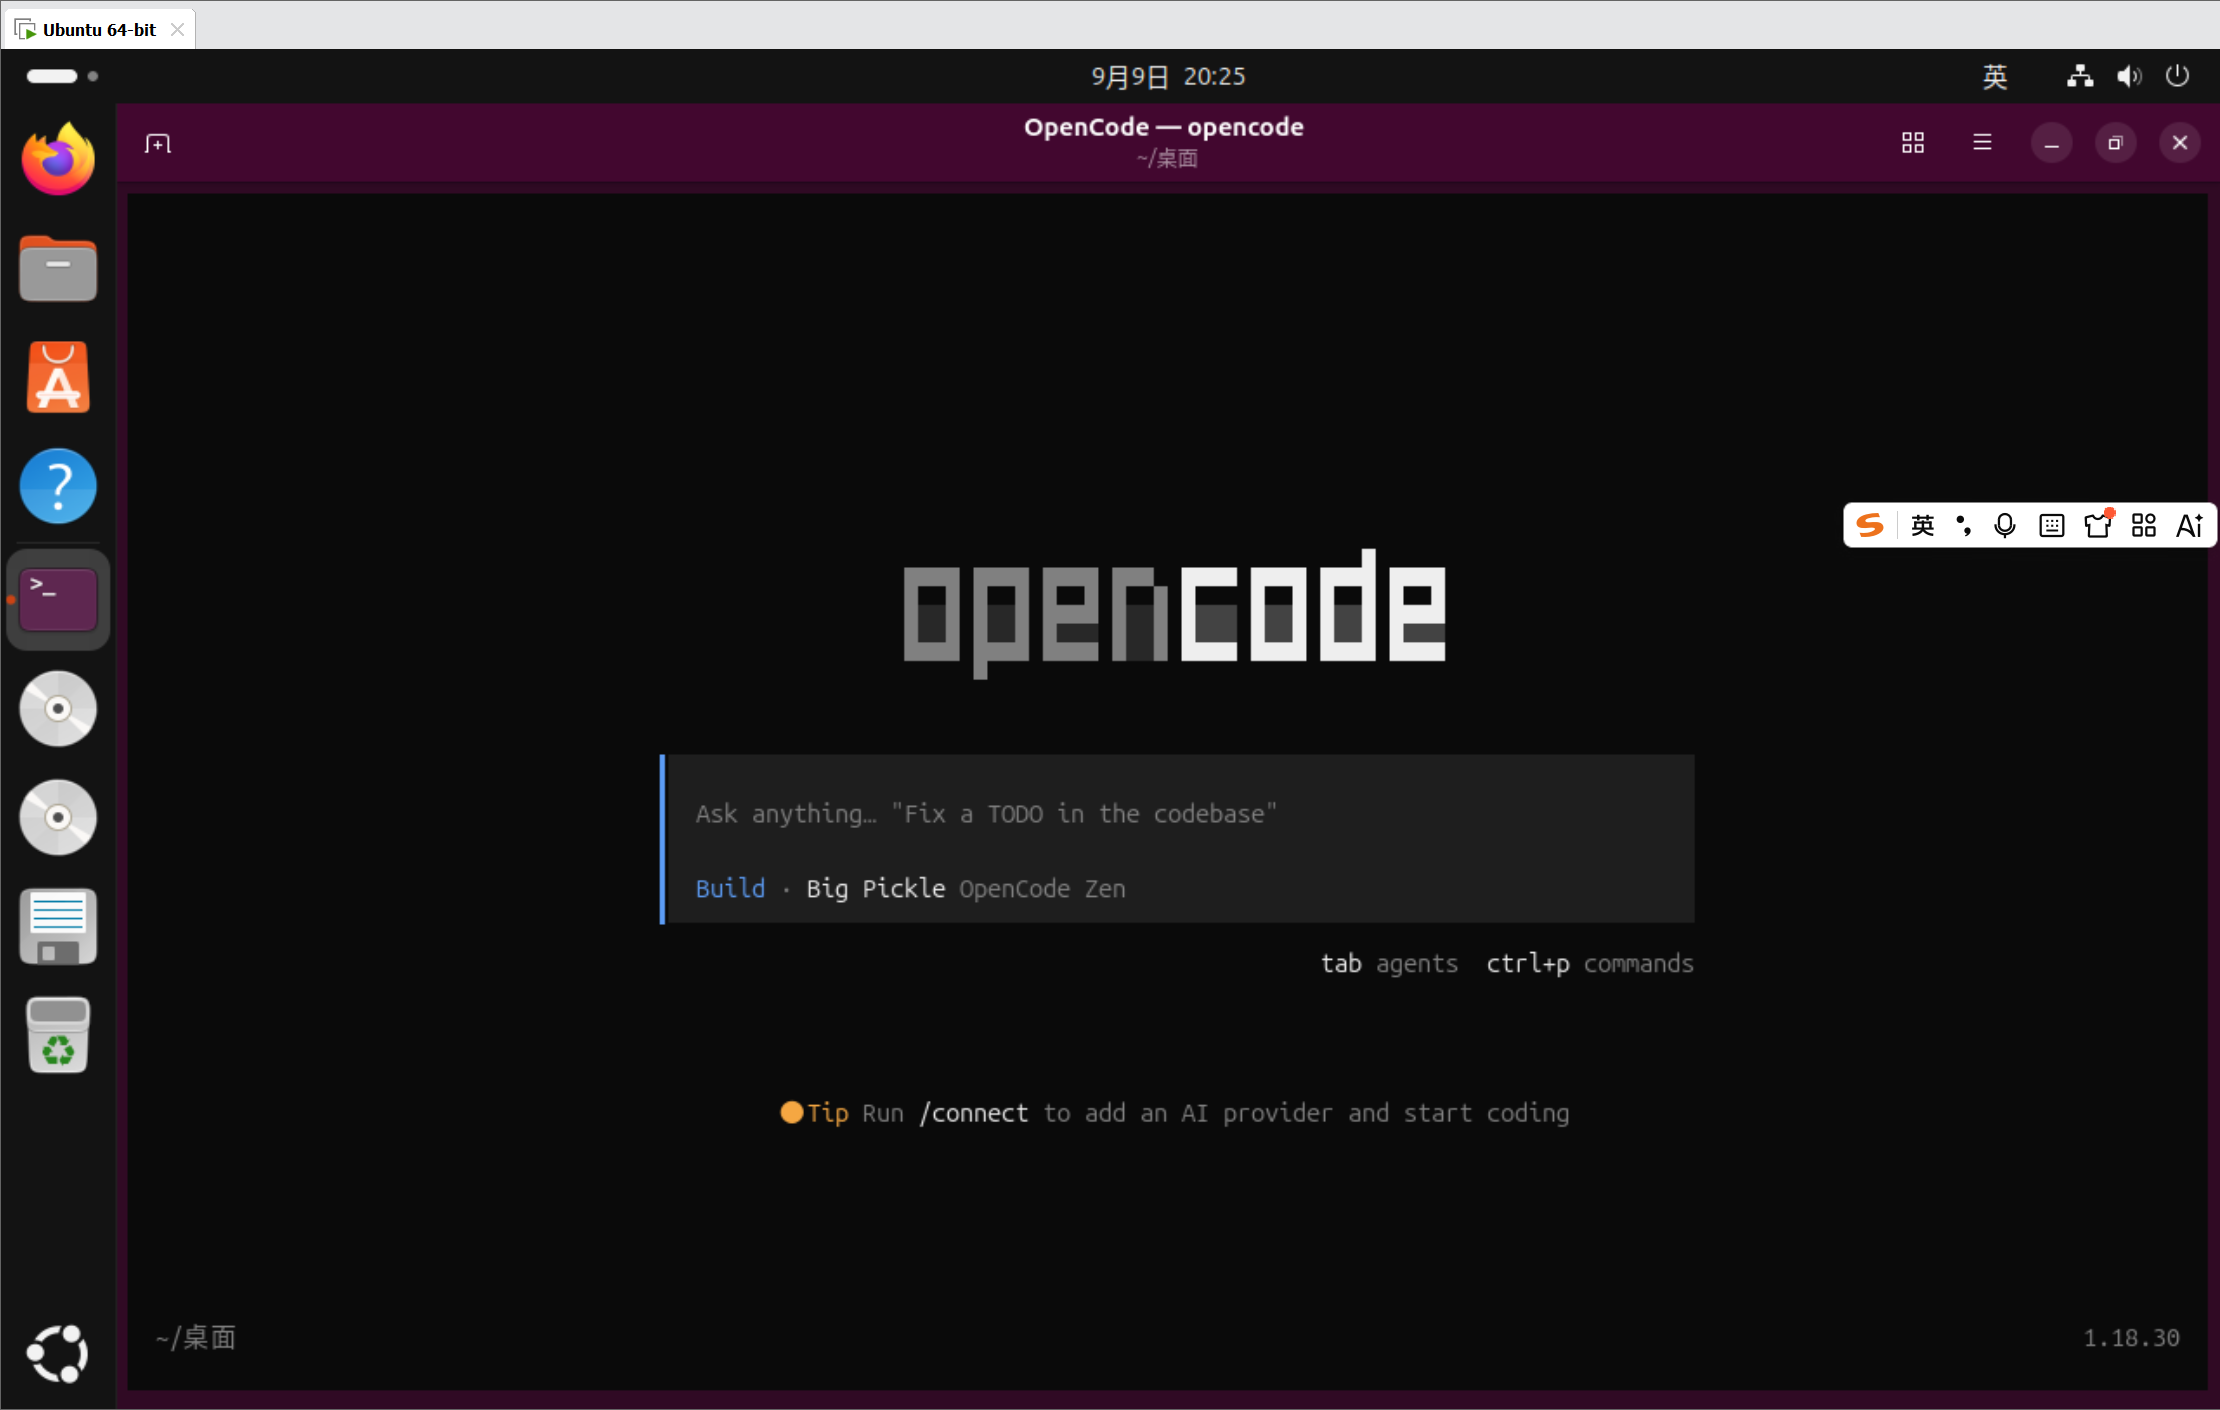
\includegraphics[width=0.8\textwidth]{Figure/Unbuntu中的opencode.png}
  \caption{Unbuntu中的opencode}
  \label{fig:Unbuntu中的opencode}
\end{figure}

% ============ 文件结尾 ============
% 整书模式(被 main.tex 引用): 读到这里即 \endinput 交还控制权,
% 不会执行下方的 \end{document}。
\ifcsname wholebook\endcsname
\expandafter\endinput
\fi

% 单独编译模式: 在顶层(无未闭合条件)执行 \end{document} 收尾。
\end{document}

% !TEX program = xelatex
% !TEX encoding = UTF-8
\ifcsname wholebook\endcsname
\else
\documentclass[12pt,a4paper]{ctexbook}
% ============================================================
% 共享导言区 preamble.tex
% 本文件被 main.tex(整书编译)和各章文件(单独编译)共同引用,
% 从而保证两种编译方式下的宏包与样式完全一致。
% 注意: 本文件不含 \documentclass, 只放宏包与样式设置。
% ============================================================
\usepackage[a4paper,margin=1.1in]{geometry}
\usepackage{graphicx}
\usepackage{listings}
\usepackage{xcolor}
\usepackage[hidelinks]{hyperref}
\usepackage{tikz}
\usetikzlibrary{positioning,arrows.meta,decorations.pathreplacing,calc}
\usepackage{booktabs}

% 代码环境样式设置
\lstset{
    basicstyle=\ttfamily\small,
    keywordstyle=\color{blue}\ttfamily,
    commentstyle=\color{gray}\ttfamily,
    stringstyle=\color{red}\ttfamily,
    backgroundcolor=\color{gray!8},
    frame=single,
    rulecolor=\color{gray!40},
    breaklines=true,
    showstringspaces=false,
    columns=fullflexible,
    keepspaces=true,
    % 允许中文注释/内容正常显示
    extendedchars=true,
    literate={
        {·}{{\cdot}}1
    }
}

\begin{document}
\fi

\chapter{Ubuntu环境下编程}
做机器人最常用的两门语言就是C++和Python，同时这两门语言也是编程语言流行度排行榜数一数二的。然后这两门咱们都学过。C++是课上教的，python语法极其简单，不赘述了。

一般用Linux的都是程序员里的大佬，都是大佬了，一般就喜欢拿记事本grdit写代码，因为不用打开编辑器，全程可以在命令行终端里执行。Linux里面还有逆天Vim，但此等极道帝兵显然不是我等炼气期小辈能够掌握的。以后编程估计都在VS code里完成，但是先看一下Ubantu里面程序的运行和编写和Windows下有何不同。
\section{Hello weijianguizhou！}
\subsection{C++}
打开终端，创建一个d2lros2文件夹接着在文件夹下创建chapt1文件夹。
然后输入这行命令：
\begin{lstlisting}[language=bash,title={用gedit创建并打开cpp文件}]
    gedit hello_weijianguizhou.cpp
\end{lstlisting}
输入：
\begin{lstlisting}[language=c++,title={cpp程序}]
    # include <iostream>
    using namespace std;
    int main(){
    	cout<<"Hello weijianguizhou!"<<endl;
    	return 0;
    }
\end{lstlisting}
保存代码，关闭gedit。

C++代码必须经过编译构建之后才能运行

C++的编译工具使用的是g++，默认是不安装的，所以我们需要手动安装一下g++。
\begin{lstlisting}[language=bash,title={安装g++编译器}]
    sudo apt install g++
\end{lstlisting}
接着在终端输入下面的指令对刚刚的代码进行编译。
\begin{lstlisting}[language=bash,title={编译C++}]
    g++ hello_weijianguizhou.cpp
\end{lstlisting}
接着使用ls指令，应该可以看到一个叫做a.out的文件。恭喜，现在可以运行了。
\begin{lstlisting}[language=bash,title={运行C++}]
    ./a.out
\end{lstlisting}
可以看出区别了。Windows系统中的可执行文件为.exe，而Linux系统中的可执行文件为.out.

真尼玛麻烦。

\subsection{python}
然后输入这行命令：
\begin{lstlisting}[language=bash,title={用gedit创建并打开py文件}]
    gedit hello_weijianguizhou.py
\end{lstlisting}
输入
\begin{lstlisting}[language=python,title={py程序}]
print("Hello weijianguizhou!")
\end{lstlisting}
保存代码，关闭gedit。
直接运行：
\begin{lstlisting}[language=bash,title={运行py}]
    python3 hello_weijianguizhou.py
\end{lstlisting}

下面看一下python和C++对比。
\begin{figure}[htbp]
  \centering
  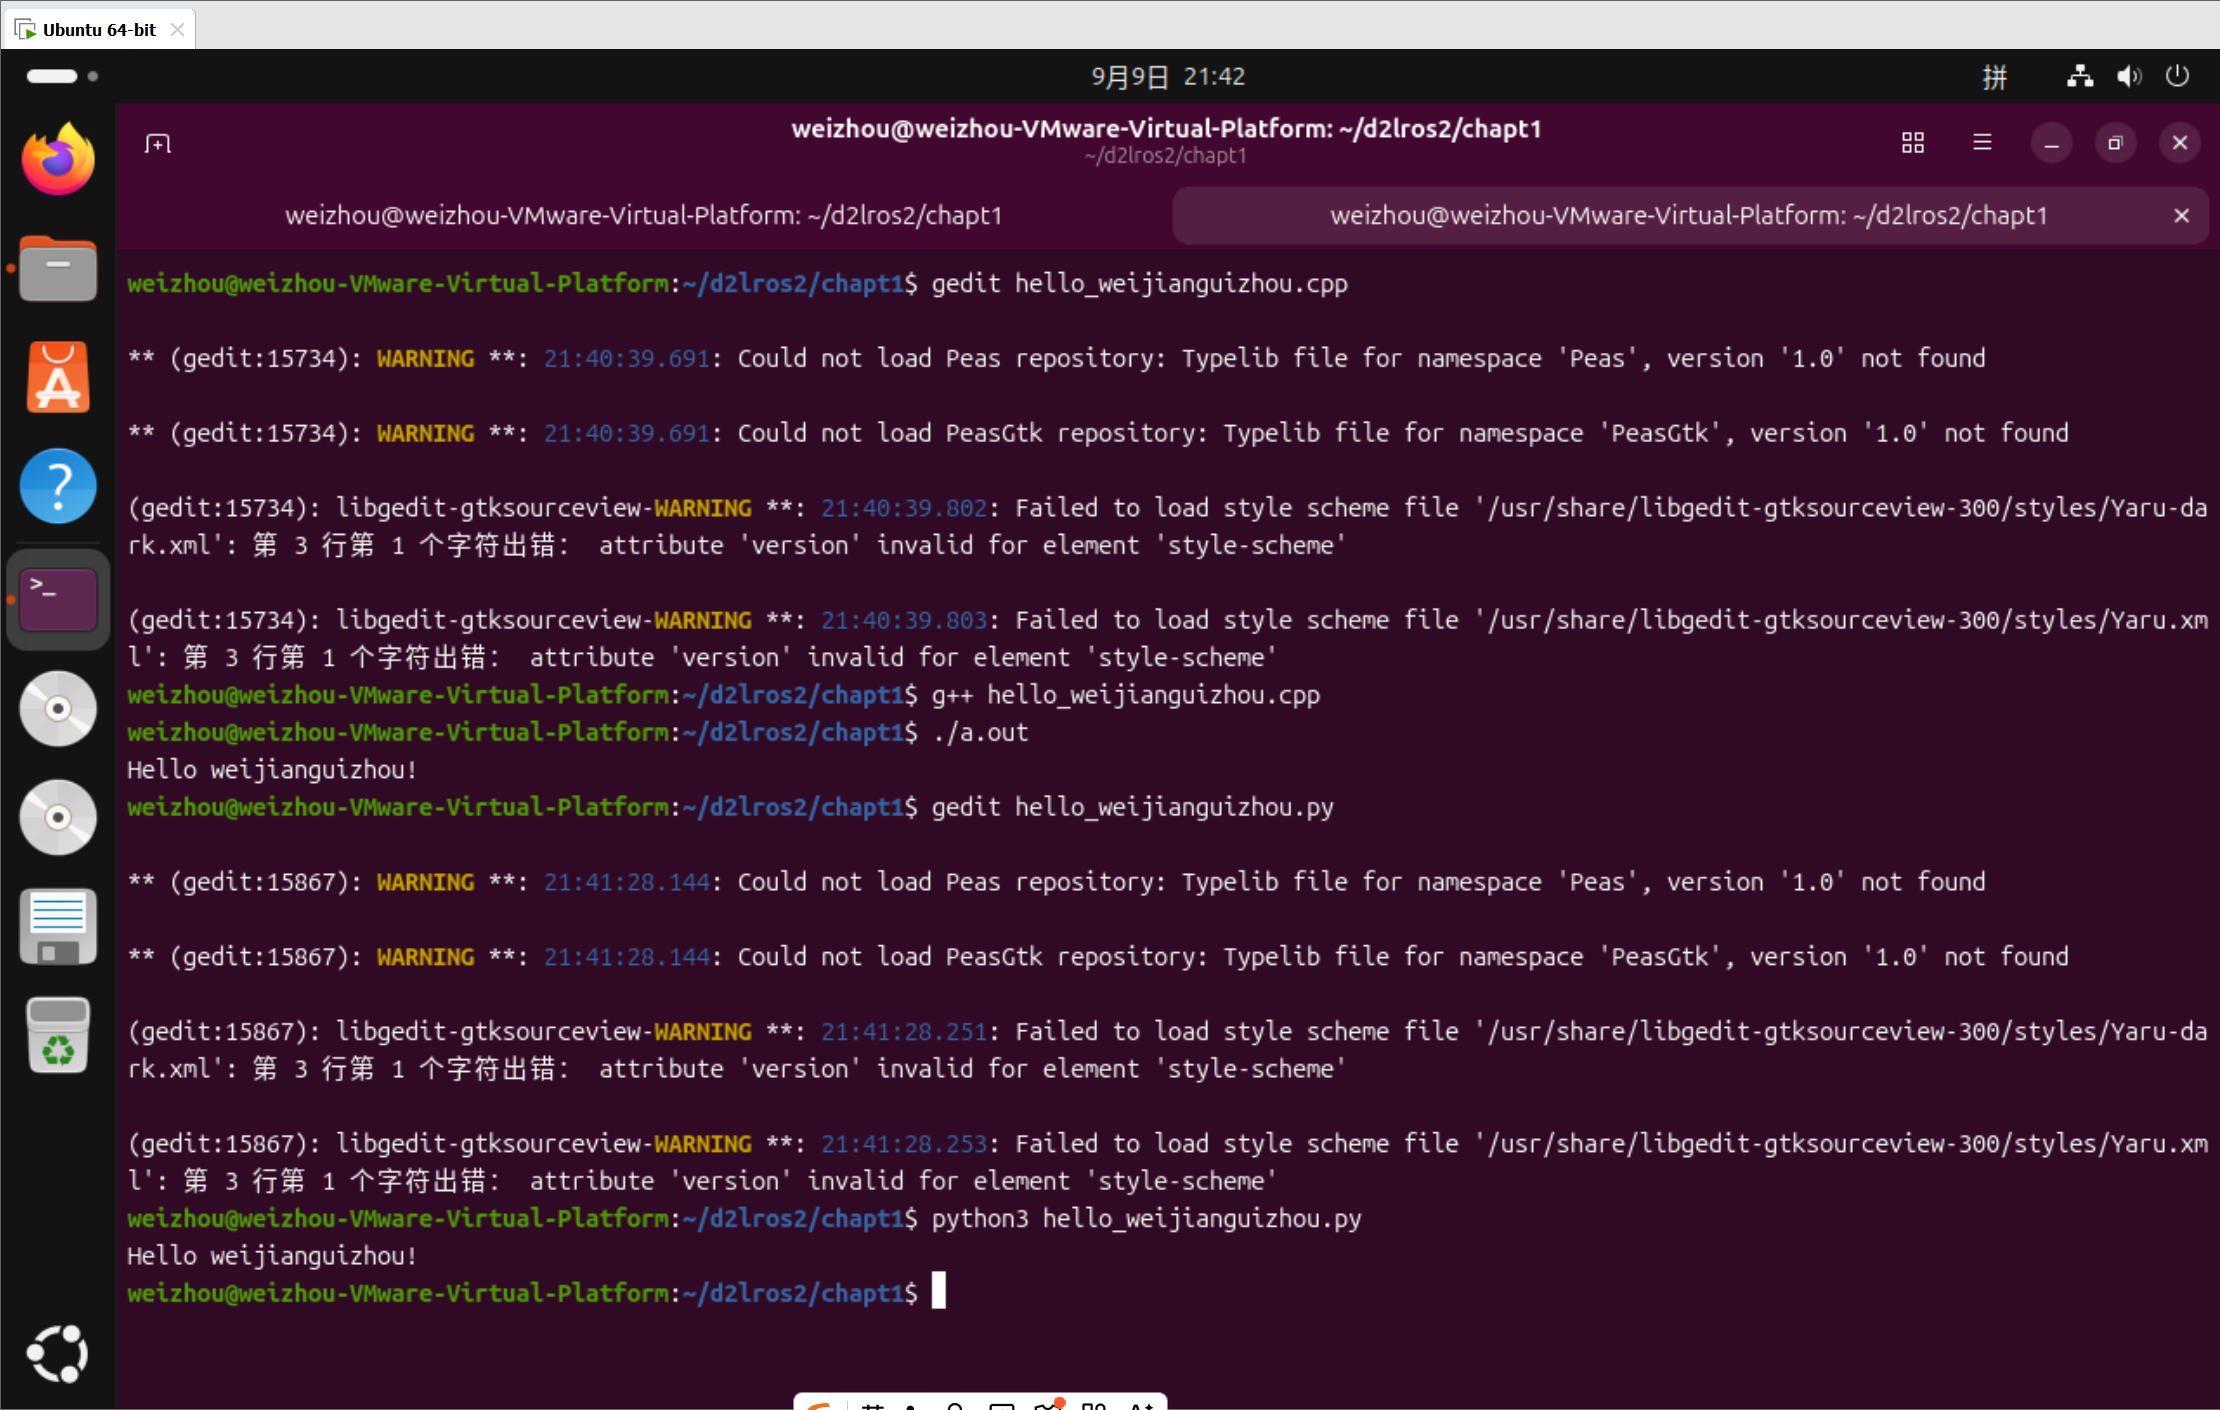
\includegraphics[width=0.8\textwidth]{Figure/python和C++对比.png}
  \caption{python和C++对比}
  \label{fig:python和C++对比}
\end{figure}
由此看来，python相比C++有如下优势：

一、python程序比C++简单。C++要6行才能搞定的程序我python只要1行就能搞定，此乃一胜。

二、python在命令行中的运行比C++简单。C++最短要三行，而我python只要一行，此乃二胜。

三、python语法更接近自然语言。此乃三胜。

由此看来，python大获全胜......吗？？？

并非啊！虽然python好用，但是它，慢啊！！！

为啥？

因为C++ 是编译执行，而python是解释执行。

\section{什么是编译执行和解释执行}
语言本身用解释型语言还是编译型语言来划分就是不准确的。

设计语言的人，也不会考虑先考虑什么型，而是在设计中发现某种方式更好，便会选择使用。语言属于XX型是呈现给大家的一个印象。

编程语言，是程序员们操控电脑以实现各种功能的主要方式，而解释执行与编译执行，是计算机编程语言的两种执行方式。

更多的时候，某个语言使用到了编译执行也用到了解释执行。

现在来笼统解释一下。
\begin{itemize}
    \item 编译：将源代码一次性转换为机器码的过程（机器码有保存为文件，下次运行的时候直接运行机器码）
    \item 解释：将源代逐行转换为机器码并运行的过程（机器码并没有保存下来）
    \item 编译执行（编译器）：将一段程序直接翻译成机器码(对于C/C++这种非跨平台的语言)或者中间码(Java这种跨平台语言，需要JVM再将字节码编译成机器码)。编译执行是直接将所有语句都编译成了机器语言，并且保存成可执行的机器码。执行的时候，是直接进行执行机器语言，不需要再进行解释/编译。
    \item 解释执行（解释器）：在执行程序时，再将中间码（例如Java的字节码通过JVM解释成机器码）一行行的解释成机器码进行执行。这个运行过程是解释一行，执行一行。
\end{itemize}

执行编译过程的程序叫做编译器。

执行解释过程的程序叫做解释器。

王垠所说的编译型语言和解释型语言的本质都是解释执行的。

编译型和解释型的语言之所以可以说相同，是因为这些语言从文本形式的源代码到最终产生的结果，所经历的过程是一样的。

根本区别是运行时，解释型需要将程序解释成机器码来运行，并没有保存机器码，是在运行过程中进行。

而编译型在运行之前就已经让编译器给程序编译成机器码了。

这也是为什么编译运行会比解释运行快的根本原因。

在知乎上看到一个比喻，非常好。

编译相当于做好了一桌子菜，可以直接开吃了。

而解释就相当于吃火锅，需要一边煮一边吃。

那么自然，吃的效率也会低一些。


\ifcsname wholebook\endcsname
\expandafter\endinput
\fi

% 单独编译模式: 在顶层(无未闭合条件)执行 \end{document} 收尾。
\end{document}
% !TEX program = xelatex
% !TEX encoding = UTF-8
\ifcsname wholebook\endcsname
\else
\documentclass[12pt,a4paper]{ctexbook}
% ============================================================
% 共享导言区 preamble.tex
% 本文件被 main.tex(整书编译)和各章文件(单独编译)共同引用,
% 从而保证两种编译方式下的宏包与样式完全一致。
% 注意: 本文件不含 \documentclass, 只放宏包与样式设置。
% ============================================================
\usepackage[a4paper,margin=1.1in]{geometry}
\usepackage{graphicx}
\usepackage{listings}
\usepackage{xcolor}
\usepackage[hidelinks]{hyperref}
\usepackage{tikz}
\usetikzlibrary{positioning,arrows.meta,decorations.pathreplacing,calc}
\usepackage{booktabs}

% 代码环境样式设置
\lstset{
    basicstyle=\ttfamily\small,
    keywordstyle=\color{blue}\ttfamily,
    commentstyle=\color{gray}\ttfamily,
    stringstyle=\color{red}\ttfamily,
    backgroundcolor=\color{gray!8},
    frame=single,
    rulecolor=\color{gray!40},
    breaklines=true,
    showstringspaces=false,
    columns=fullflexible,
    keepspaces=true,
    % 允许中文注释/内容正常显示
    extendedchars=true,
    literate={
        {·}{{\cdot}}1
    }
}

\begin{document}
\fi

\chapter{ROS2基础}
\section{ROS2的下载}
首先启动虚拟机中的ubuntu，打开终端，输入下面的指令。
\begin{lstlisting}[language=bash,title={一键安装指令}]
    wget http://fishros.com/install -O fishros && . fishros
\end{lstlisting}
输入密码，在选项界面选择1-一键安装ROS，接着根据你的情况选择是否更换系统源，接着等待一会就会让你选择要安装的ROS2版本了。这里选择humble版本的ROS2即可。

接着会问你安装桌面版还是基础版，我们选择桌面版，包含可视化工具，嗯，我就喜欢可视化工具，如果是在树莓派上装可以使用基础版。

安装完成后输入ros2如果看到下面的界面则安装成功。
\begin{figure}[h]
  \centering
  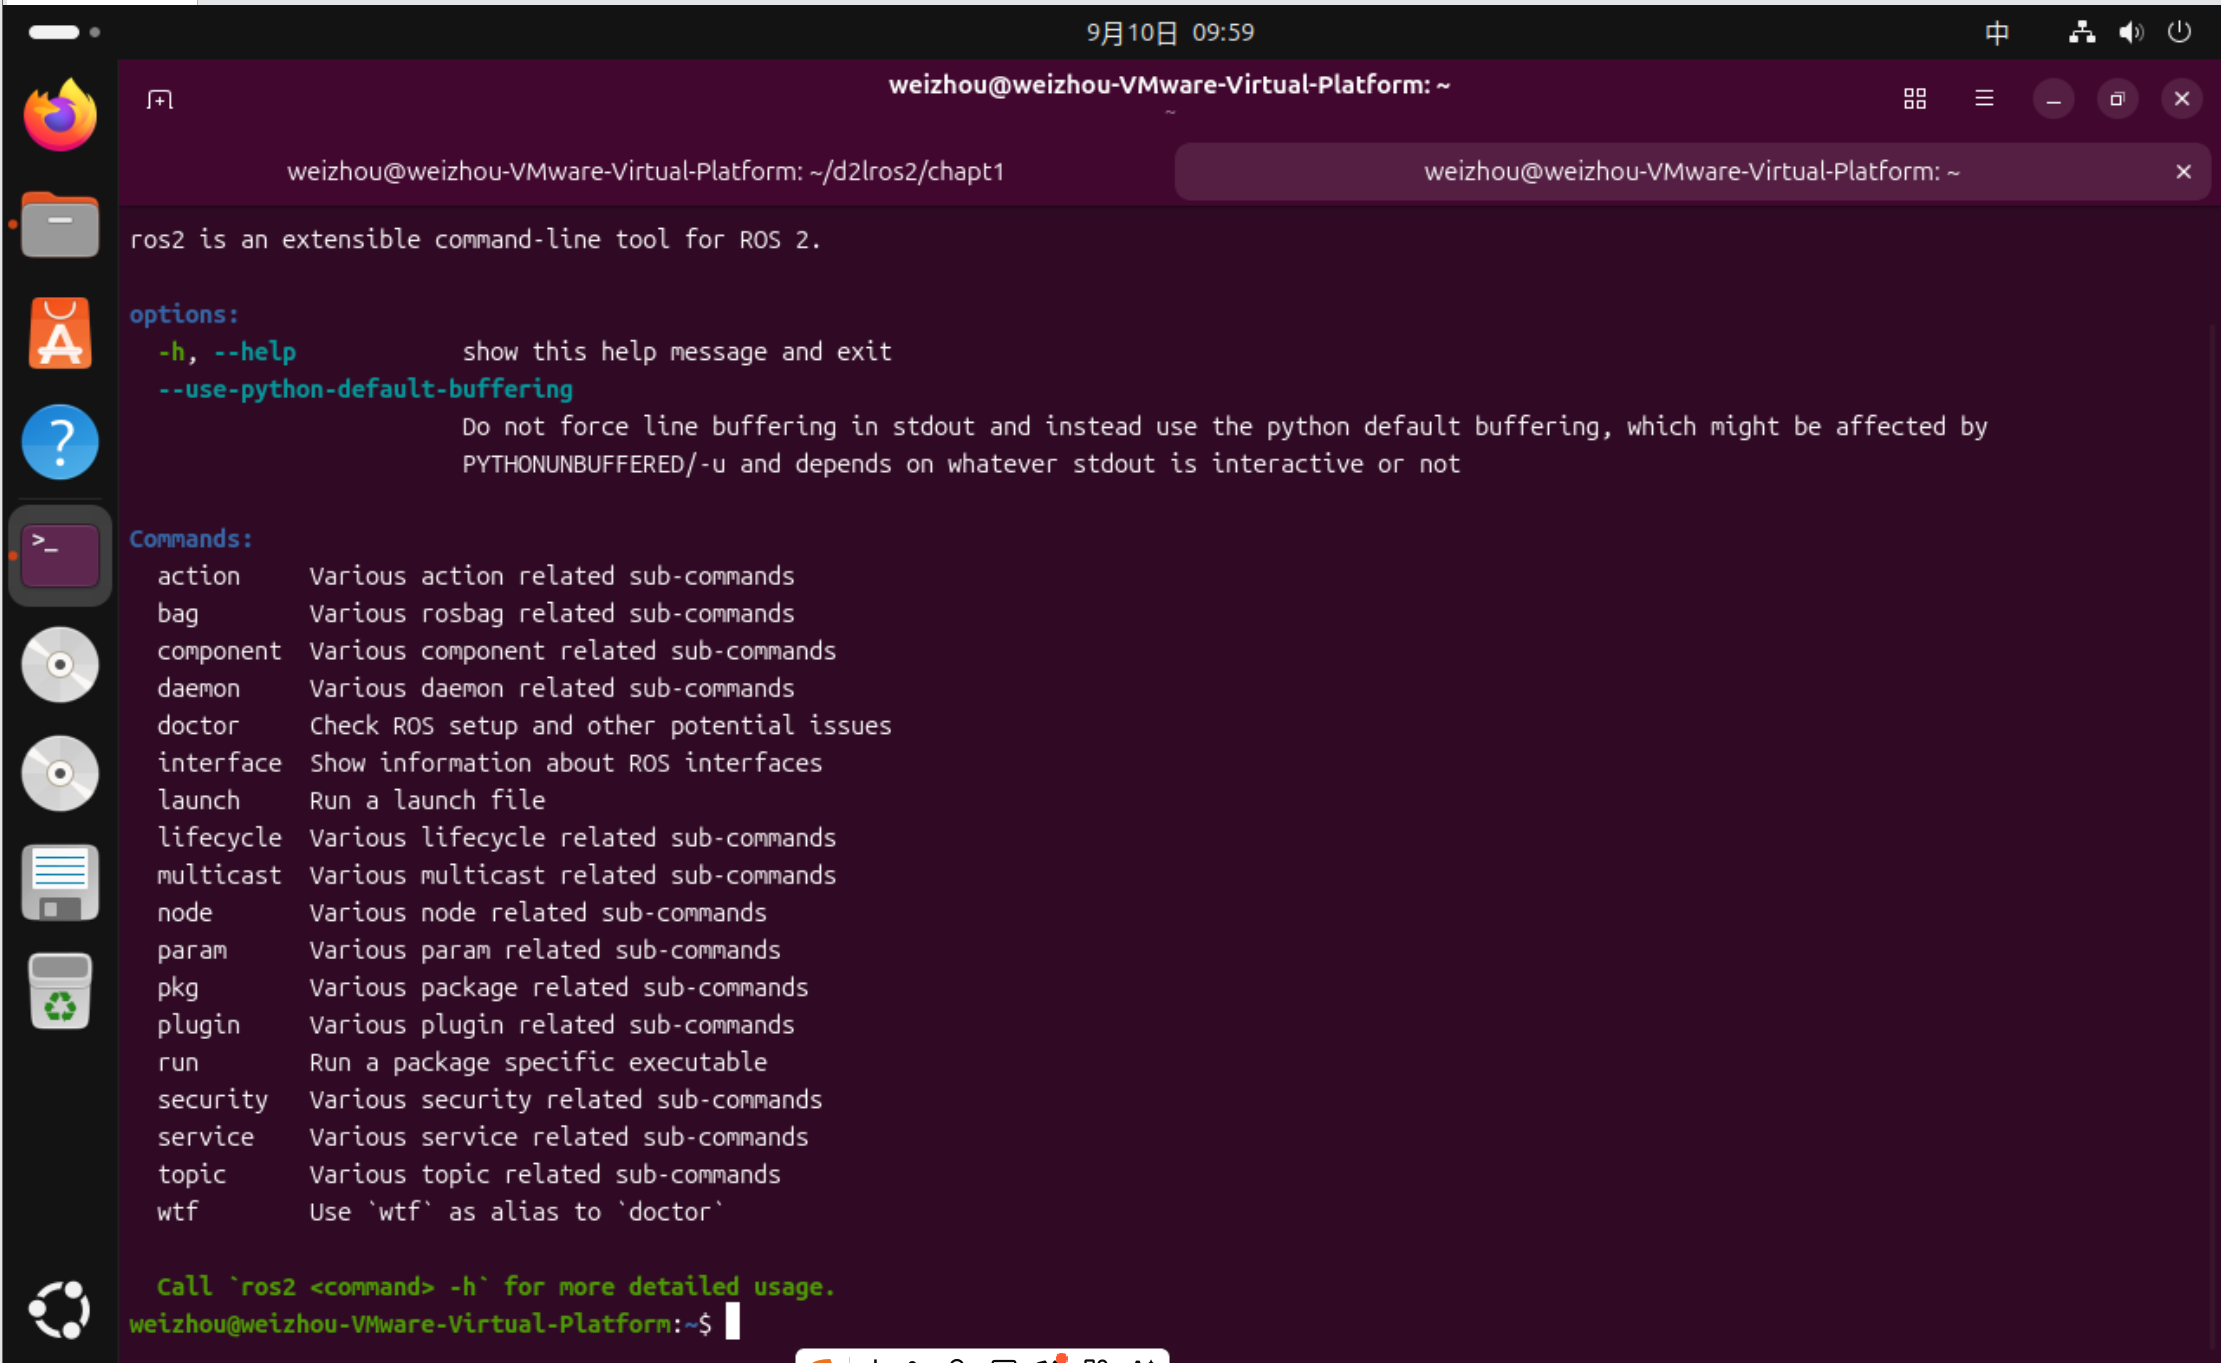
\includegraphics[width=0.8\textwidth]{Figure/ROS2成功安装界面.png}
  \caption{ROS2成功安装界面}
  \label{fig:ROS2成功安装界面}
\end{figure}

那要是我瞎玩，给ROS2环境弄乱了。该怎么办呢？删掉重装就好了呀。
\begin{lstlisting}[language=bash,title={一键卸载ROS2}]
    sudo apt remove ros-humble-*
    sudo apt autoremove
\end{lstlisting}

我们都知道安装软件要设置安装目录。那么ROS2装在哪里了呢？ROS安装的默认目录在/opt/ros/下，根据版本的名字进行区分。安装的是humble版本的ROS，所以安装目录在/opt/ros/humble下。

\section{ROS2体验}
\subsection{你说我听}
游戏内容：很简单，我们启动两个节点，一个节点负责发消息(说)，一个节点负责收消息（听）。
\begin{enumerate}
    \item 启动一个终端，快捷键 \texttt{Ctrl+Alt+T}。
    \item 在终端中启动倾听者：\verb|ros2 run demo_nodes_py listener|
    \item 再启动一个新终端，快捷键 \texttt{Ctrl+Alt+T}。
    \item 在新终端中启动说话者：\verb|ros2 run demo_nodes_cpp talker|
\end{enumerate}
观察一下现象，talker节点每数一个输，倾听节点每一次都能听到一个，是不是很神奇。
\begin{figure}[h]
  \centering
  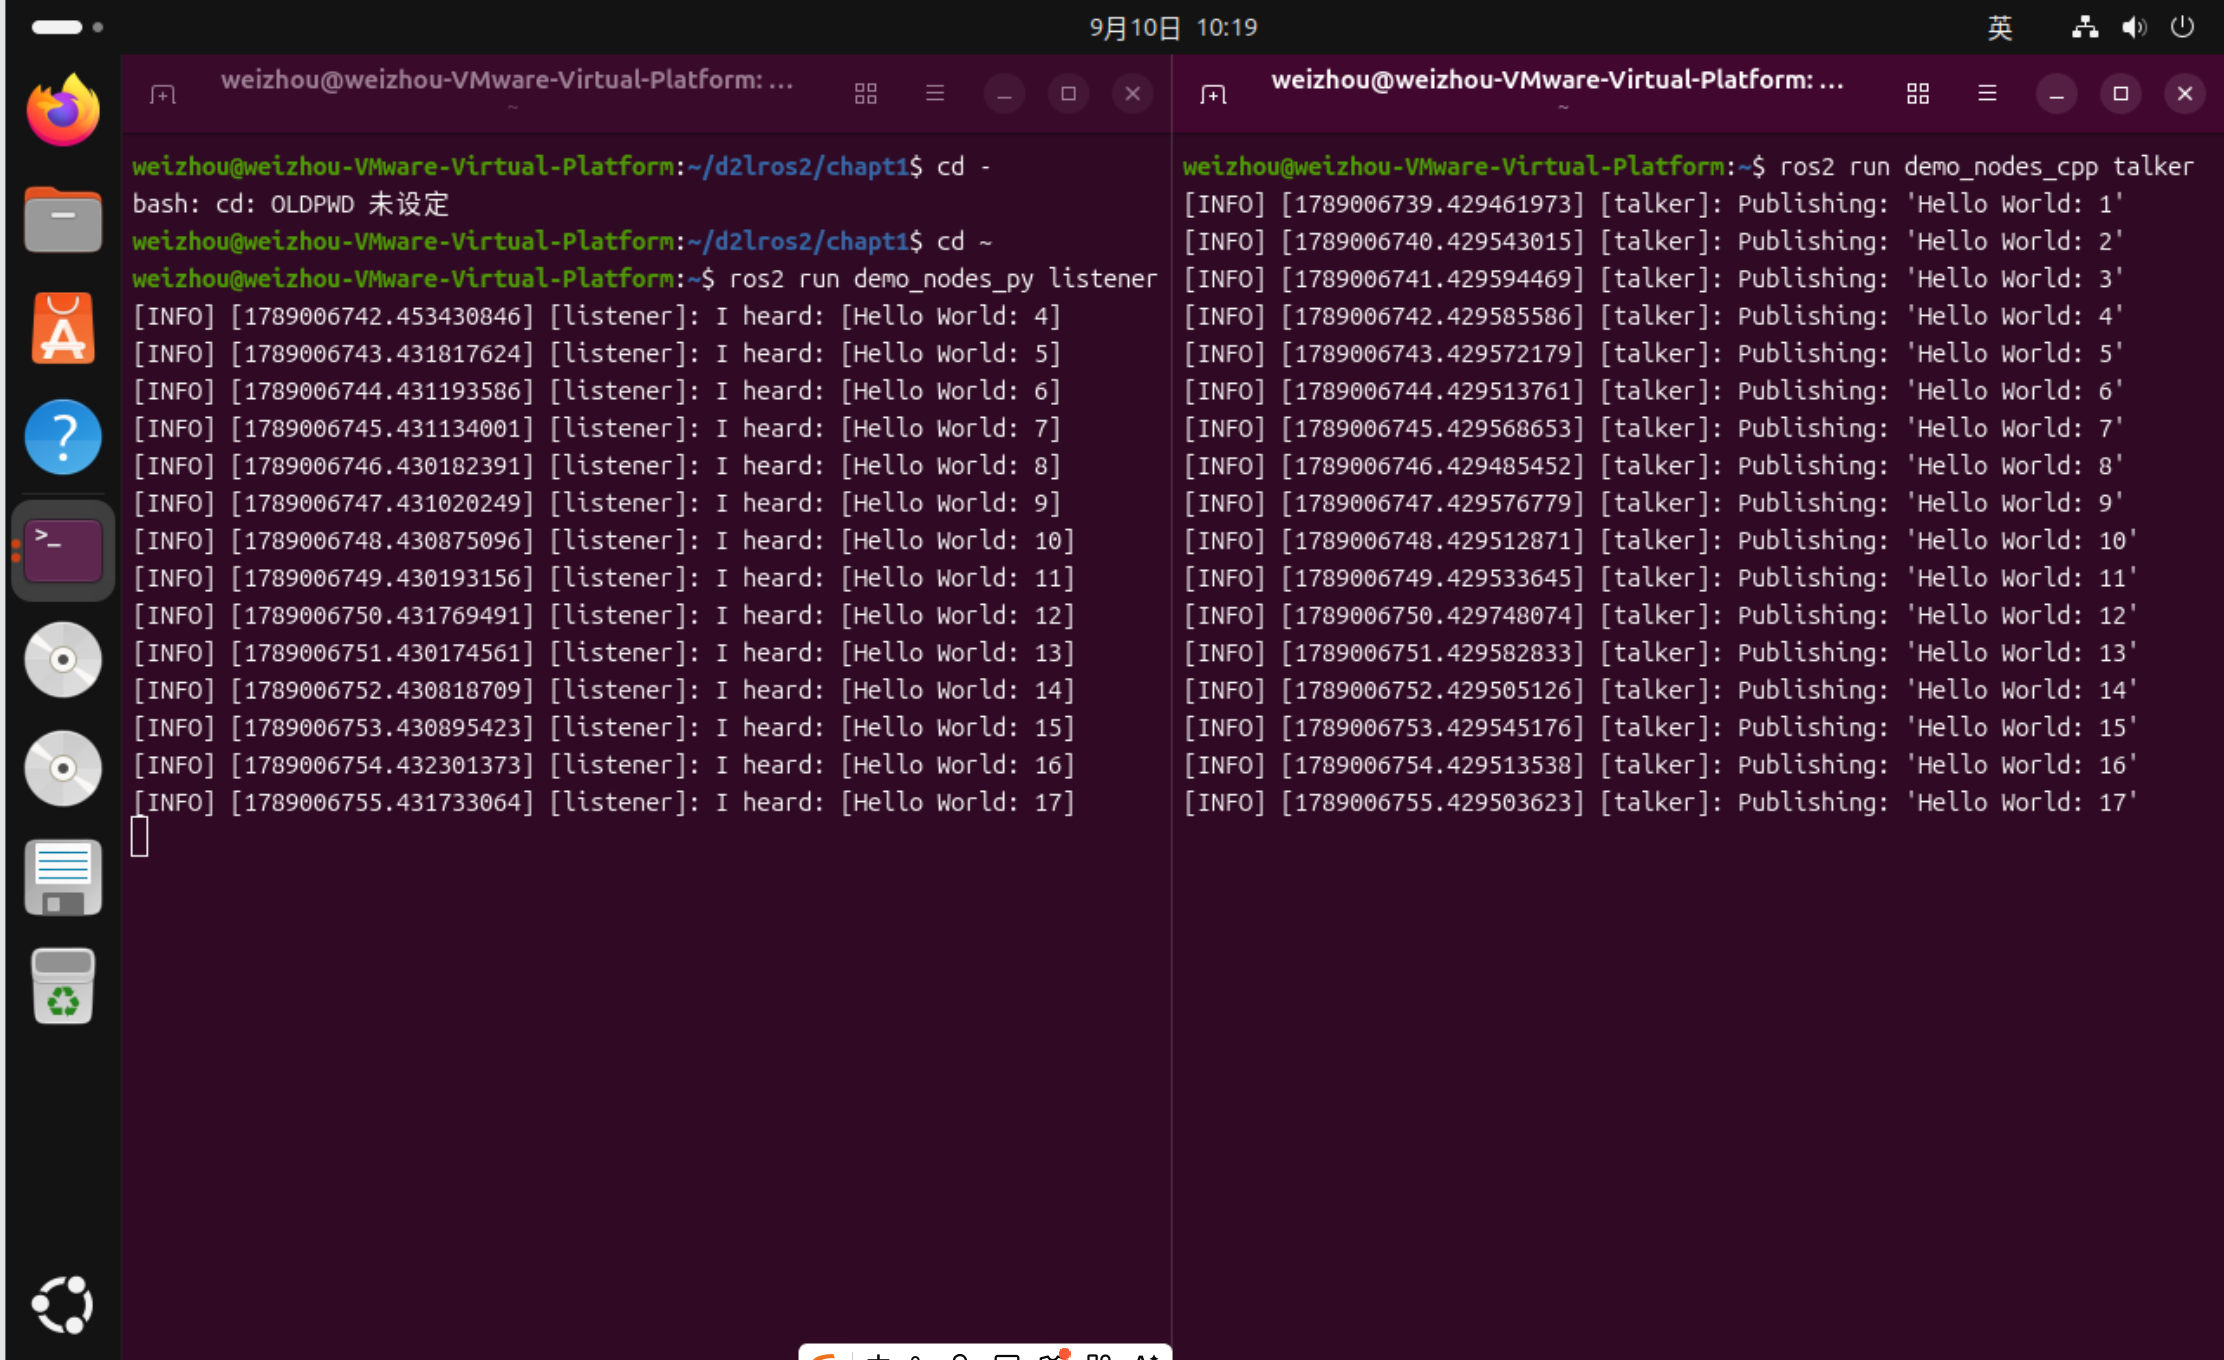
\includegraphics[width=0.8\textwidth]{Figure/你说我听.png}
  \caption{你说我听}
  \label{fig:你说我听}
\end{figure}

\subsection{涂鸦乌龟}
打开终端Ctrl+Alt+T,输入下面的指令
\begin{lstlisting}[language=bash,title={启动海龟画图}]
    ros2 run turtlesim turtlesim_node
\end{lstlisting}
如下图所示：
\begin{figure}[h]
  \centering
  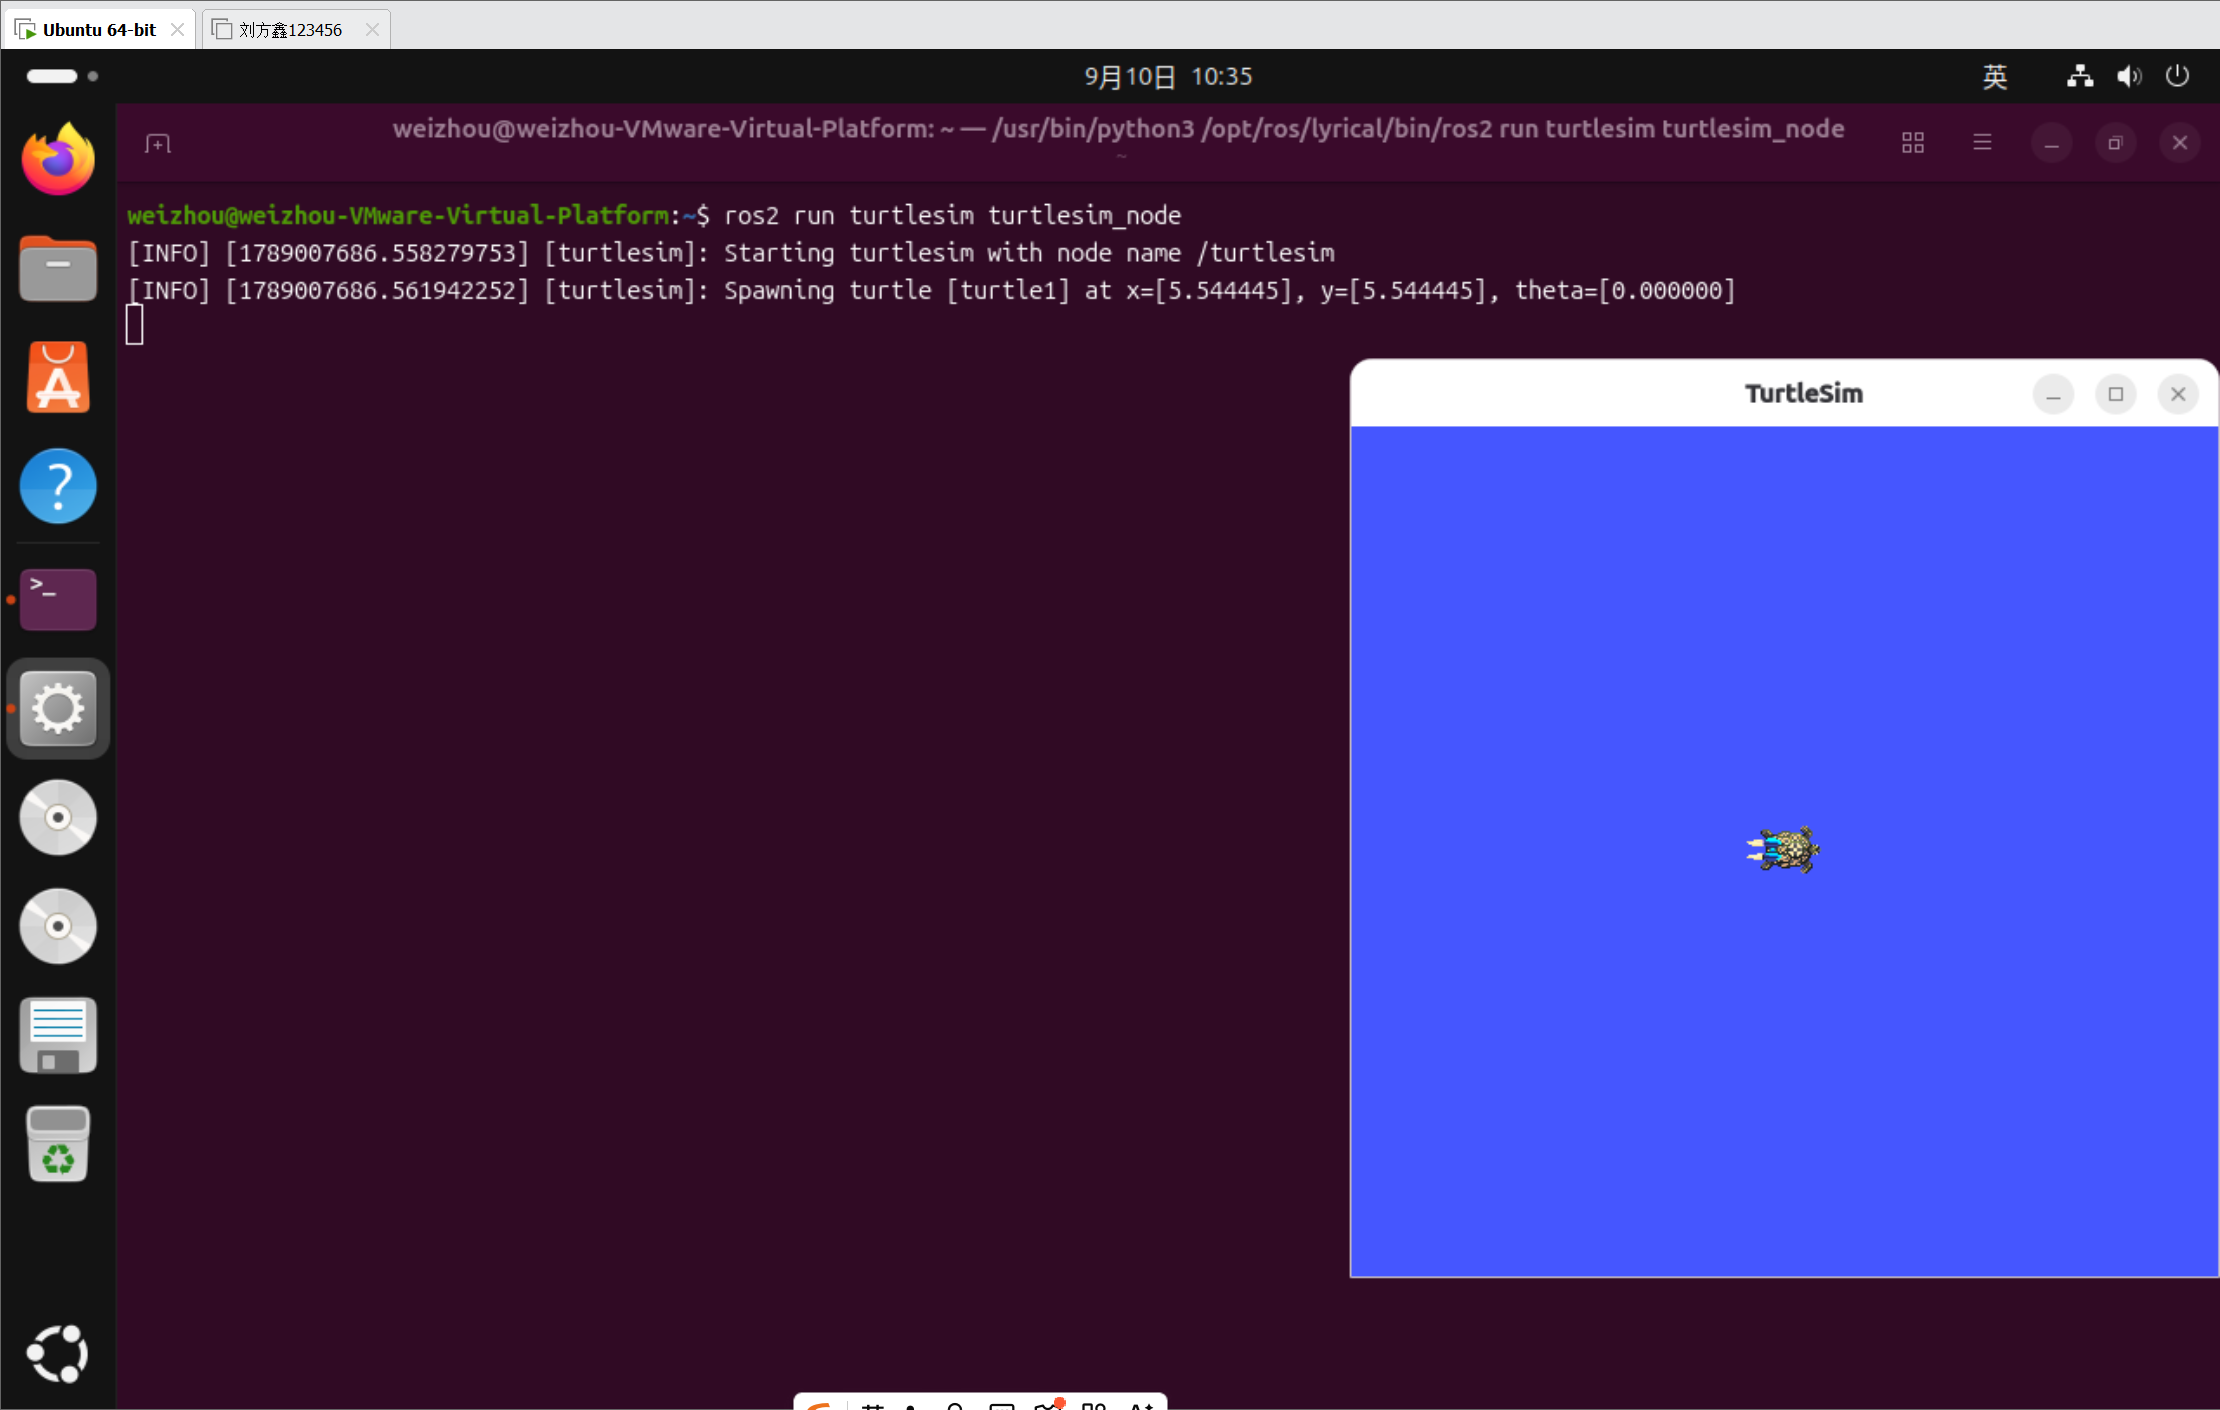
\includegraphics[width=0.8\textwidth]{Figure/海龟模拟器}
  \caption{海龟模拟器}
  \label{fig:海龟模拟器}
\end{figure}

点一下原来的终端输入Ctrl+Shift+T 打开一个新的标签页输入
\begin{lstlisting}[language=bash,title={启动海龟操控}]
    ros2 run turtlesim turtle_teleop_key
\end{lstlisting}
\newpage
\subsection{RQT可视化}
保持前面两个游戏在运行状态，打开终端，输入rqt。
打开之后选择插件Introspection / Node Graph，刷新一下，即可看见两个节点间的通信关系。
\begin{figure}[h]
  \centering
  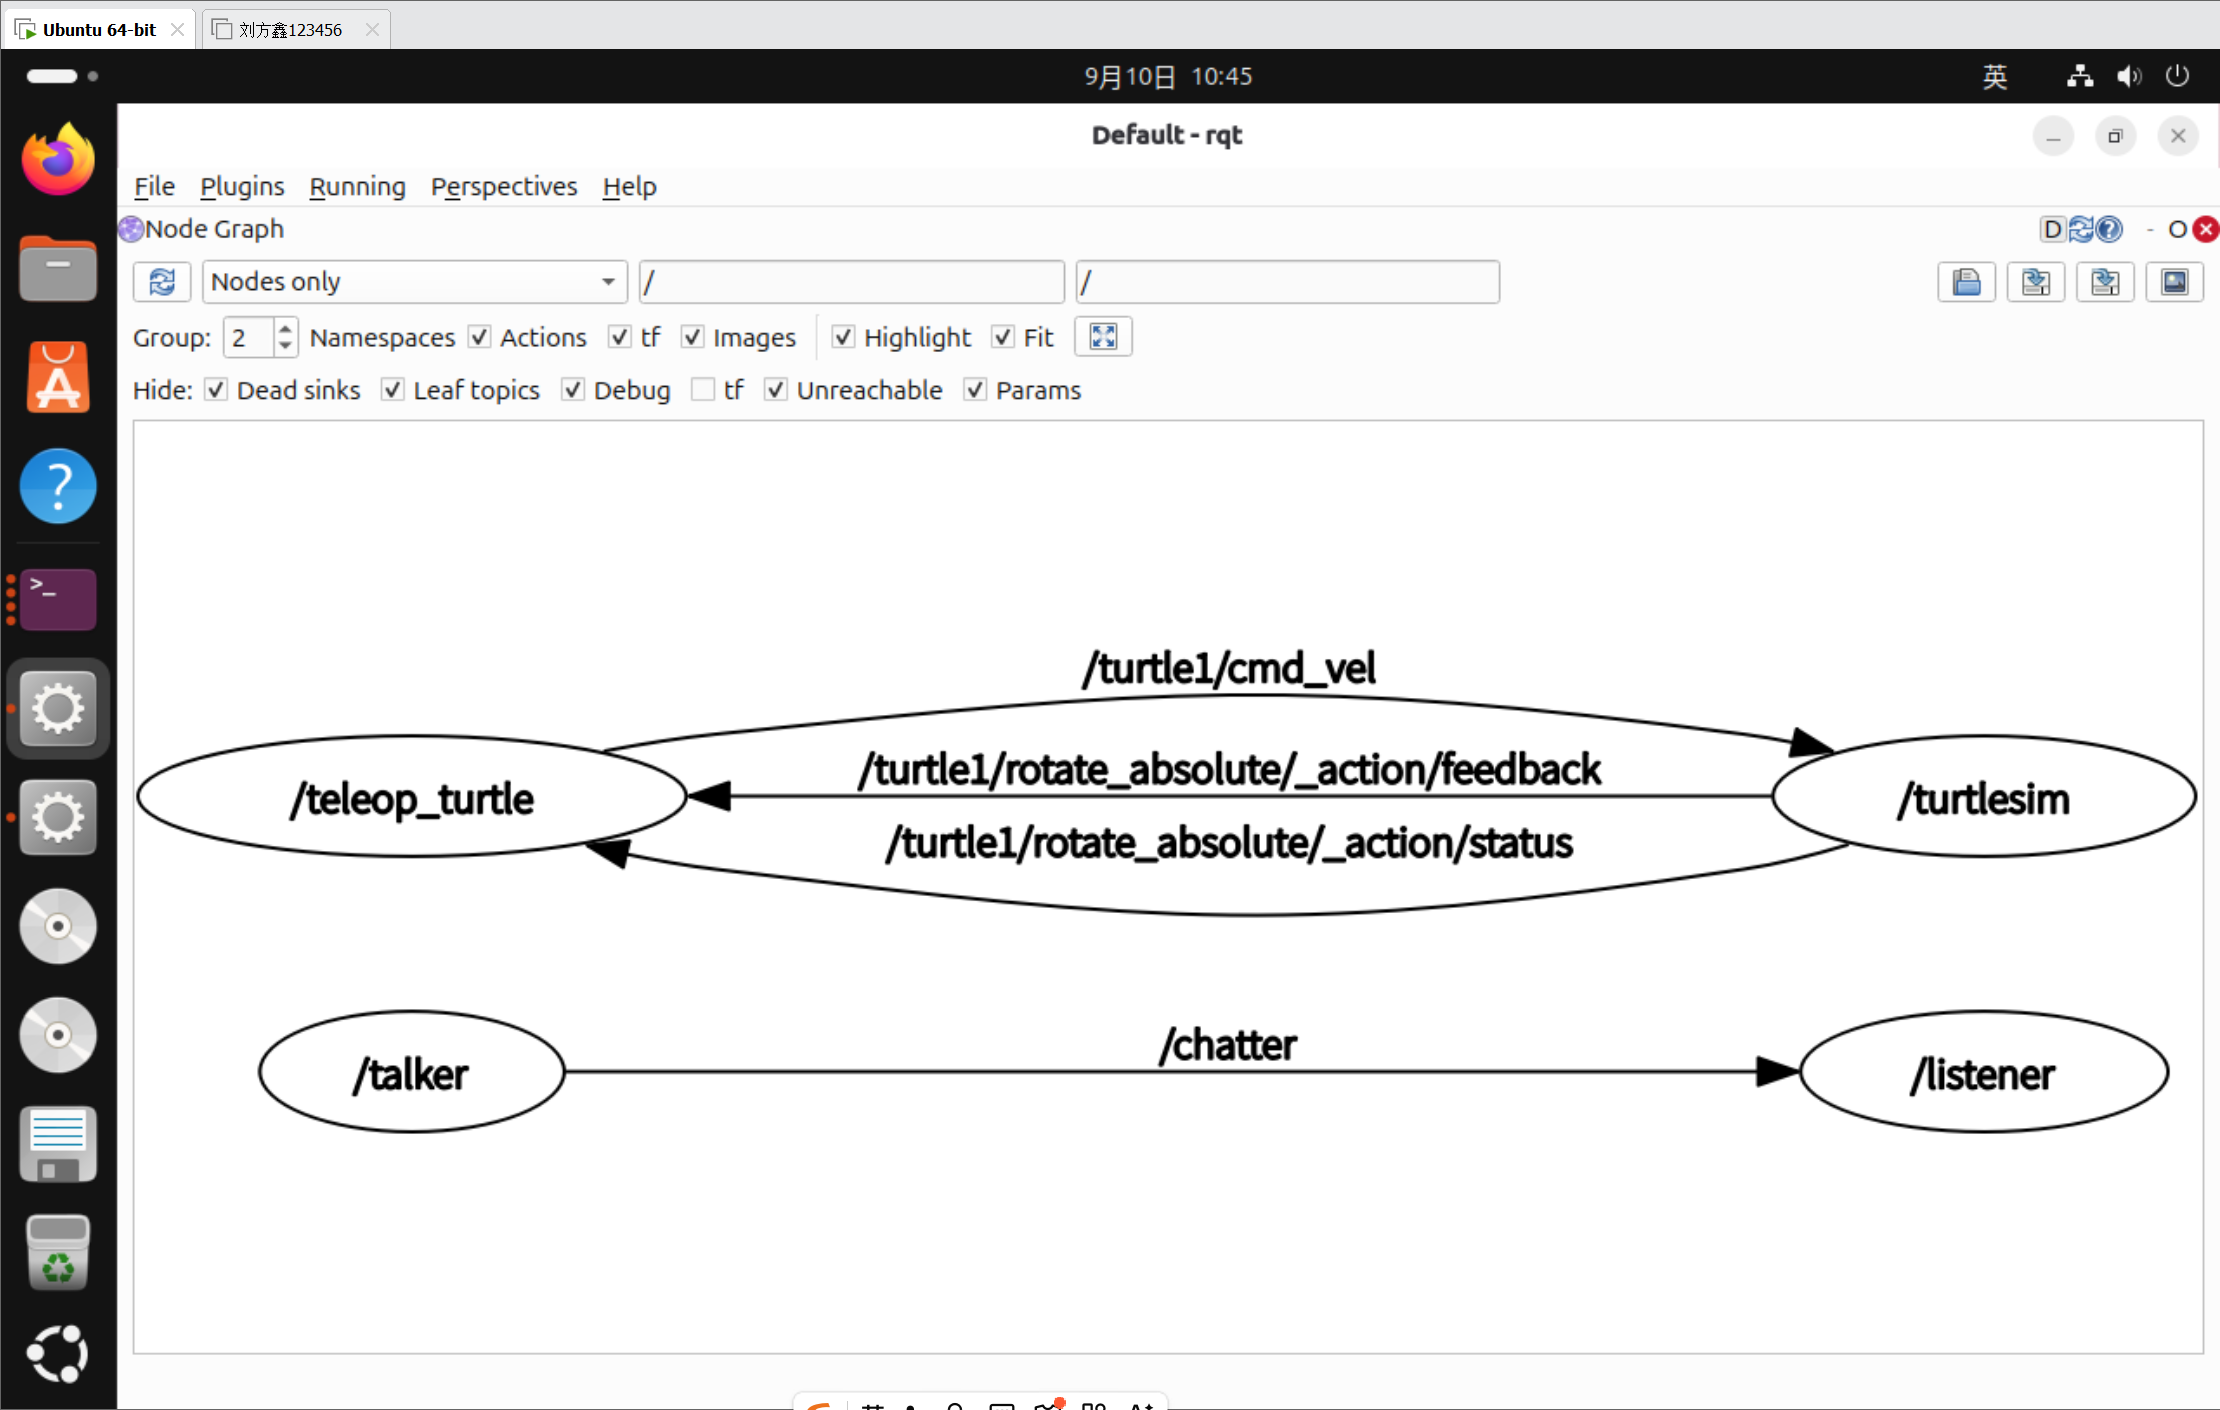
\includegraphics[width=0.8\textwidth]{Figure/RQT Node Graph 可视化.png}
  \caption{RQT Node Graph 可视化}
  \label{fig:RQT Node Graph 可视化}
\end{figure}

\section{ROS2系统架构}
前面两个小游戏你已经玩过了，节点能跑起来，rqt 里也能看到它们之间的连线。不过这些都还停留在“会用”的层面。这一节我们把 ROS2 拆开，从整体框架上看一看它到底由哪几层构成，以及为什么要这样分层。

\subsection{分层架构总览}
ROS2 的整体结构可以用一张“千层饼”式的图来描述，从上到下依次是：应用层、ROS2 客户端库、客户端库核心 rcl、中间件抽象层 RMW、DDS 实现层、操作系统层。相邻两层之间是双向的调用关系：上层向下层提出请求，下层把结果和事件回传给上层。

\begin{figure}[htbp]
\centering
\begin{tikzpicture}[font=\small,
  layer/.style={draw=black!65, rounded corners=2.5pt, minimum width=9.2cm,
                minimum height=1.05cm, align=center, text width=8.6cm, inner sep=3pt}]

\node[layer, fill=blue!10]  (app)  {应用层\\[-1pt]{\footnotesize 用户节点 · rqt · 命令行工具}};
\node[layer, fill=cyan!10,  below=4mm of app]  (rcl)  {ROS2 客户端库\\[-1pt]{\footnotesize rclpy · rclcpp · rcljava · rclnodejs · \dots}};
\node[layer, fill=teal!12,  below=4mm of rcl]  (rclc) {客户端库核心 rcl（C 语言实现）};
\node[layer, fill=orange!15,below=4mm of rclc] (rmw)  {中间件抽象层 RMW};
\node[layer, fill=red!10,   below=4mm of rmw]  (dds)  {DDS 实现层\\[-1pt]{\footnotesize Fast DDS · Cyclone DDS · Connext · \dots}};
\node[layer, fill=green!12, below=4mm of dds]  (os)   {操作系统层\\[-1pt]{\footnotesize Linux · Windows · macOS · 驱动与网络协议栈}};

\foreach \a/\b in {os/dds, dds/rmw, rmw/rclc, rclc/rcl, rcl/app}{
  \draw[<->, >=stealth, thick, black!55] (\a.north) -- (\b.south);
}

\draw[decorate, decoration={brace, amplitude=4pt, mirror}, black!60]
  ($(app.north east)+(0.35,0)$) -- ($(rclc.south east)+(0.35,0)$)
  node[midway, right=7pt, align=left, font=\footnotesize,
       text width=2.6cm] {ROS2 自身的实现，\\跨语言绑定};

\draw[decorate, decoration={brace, amplitude=4pt, mirror}, black!60]
  ($(rmw.north east)+(0.35,0)$) -- ($(rmw.south east)+(0.35,0)$)
  node[midway, right=7pt, align=left, font=\footnotesize,
       text width=2.6cm] {统一接口，\\屏蔽各家差异};

\draw[decorate, decoration={brace, amplitude=4pt, mirror}, black!60]
  ($(dds.north east)+(0.35,0)$) -- ($(dds.south east)+(0.35,0)$)
  node[midway, right=7pt, align=left, font=\footnotesize,
       text width=2.6cm] {第三方中间件，\\可自由替换};
\end{tikzpicture}
\caption{ROS2 的分层架构。自下而上依次是操作系统层、DDS 实现层、中间件抽象层 RMW、客户端库 RCL 以及最顶端的应用层，相邻两层之间为双向调用关系}
\label{fig:ROS2分层架构}
\end{figure}

图~\ref{fig:ROS2分层架构} 中两侧的括号标出了各层的归属：从应用层到客户端库核心 rcl，这三层是 ROS2 官方自己实现的；中间件抽象层 RMW 是统一接口；最下面的 DDS 实现层则来自第三方。接下来我们自下而上，一层一层地看。



\subsection{操作系统层}
这一层最好理解。ROS2 自己并不是一个操作系统，它只是跑在 Linux、Windows 或 macOS 之上的一个中间件框架。真正去驱动硬件、管理进程、收发底层网络数据包这些脏活累活，全部交给操作系统来完成。也正因为如此，ROS2 才能在这么多平台上跑起来：只要那个平台提供的系统调用和网络协议栈足够完整，上面的各层就可以原封不动地搬过去。

顺带说一句，我们在第一章里折腾 Ubuntu 虚拟机，其实就是在给上面的几层准备一块合适的“地基”。

\subsection{DDS 实现层}
想弄懂这一层，你得先回答两个问题：DDS 到底是什么？以及为什么 ROS2 里会同时存在好几套 DDS 实现？

\subsubsection{DDS 是什么}

DDS，全称 Data Distribution Service，中文叫“数据分发服务”，是由对象管理组 OMG（Object Management Group）在 2003 年发布、2007 年修订的一套分布式系统通信标准。

它的通信方式和 ROS 里的话题发布订阅几乎一模一样：一方把数据“发布”到某个主题上，关心这个主题的另一方“订阅”后就能收到，双方不需要事先知道对方是谁。除此之外，DDS 还提供了相当丰富的服务质量（QoS）策略，用来规定通信的可靠性、持久性、传输方式等要求。

正因为设计理念如此契合，ROS2 干脆不再自己另造一套通信协议，而是直接把 DDS 拿来当作底层的通信支柱。

\subsubsection{为什么会有多套 DDS 实现}

DDS 只是一份标准文档，标准本身不能运行，得有人照着它写出真正的程序，这些程序就叫“DDS 实现”。目前常见的实现有 eProsima 的 Fast DDS、Eclipse 的 Cyclone DDS、RTI 的 Connext DDS 等。它们遵守同一份标准，但侧重点各不相同：有的偏重性能，有的体积小巧，有的面向商用场景提供技术支持。

既然标准是统一的，那多准备几套实现就不会给上层添麻烦，想换随时换。至于这些差异是怎么被“抹平”的，就要看下面这一层了。

\subsection{中间件抽象层 RMW}
RMW 是 ROS Middleware 的缩写，也就是中间件抽象层。它的作用可以用一句话概括：\textbf{给上面一个统一的接口，把下面各家的差异藏起来}。

为什么不直接把 DDS 暴露给上层呢？因为直接用 DDS 其实挺麻烦的。创建一次通信要设置分区、主题名称、发现模式、消息类型等一大堆参数，还要记得在不用的时候逐项清理。这些琐碎而重复的配置如果让每个写节点的同学自己处理，代码会变得又臭又长。

于是 ROS2 在这中间加了一层 RMW：它定义好一套固定的接口，无论底下换成 Fast DDS 还是 Cyclone DDS，上层看到的 API 都完全一样。那些繁琐的配置也就顺理成章地在 RMW 和 RCL 里统一完成了。

\begin{lstlisting}[language=bash,title={查看与切换 DDS 实现}]
# 查看当前使用的 DDS 实现
ros2 doctor --report | grep middleware

# 通过环境变量切换（需要系统里已安装对应的 DDS）
export RMW_IMPLEMENTATION=rmw_cyclonedds_cpp
\end{lstlisting}

\subsection{客户端库 RCL 与语言绑定}
RCL 是 ROS Client Library 的缩写，也就是 ROS2 客户端库。它建立在 RMW 之上，把 ROS 里的节点、话题、服务、参数、Action 这些概念包装成一套好用的 API。

这里有个细节值得留意：RCL 的底层实现是用 C 语言写的，因为 C 是众多高级语言的“共同祖先”，基于它再去封装其它语言会轻松很多。所以官方的 rclpy（Python）和 rclcpp（C++）都是直接建立在这套 C 实现之上的。这也是为什么后面我们用两种语言写节点时，代码结构会如此相似。

社区还用同样的方式把 ROS2 搬到了更多语言和平台上，比如在 Android 应用或网页里也能和 ROS2 通信：

\begin{table}[htbp]
  \centering
  \caption{ROS2 的常见多语言客户端库}
  \label{tab:rcl-bindings}
  \small
  \begin{tabular}{@{}lll@{}}
    \toprule
    语言 & 客户端库 & 项目地址 \\
    \midrule
    Python & rclpy & \url{https://github.com/ros2/rclpy} \\
    C++ & rclcpp & \url{https://github.com/ros2/rclcpp} \\
    Java & rcljava & \url{https://github.com/esteve/ros2_java} \\
    Rust & rclrust & \url{https://github.com/ros2-rust/ros2_rust} \\
    Node.js & rclnodejs & \url{https://github.com/RobotWebTools/rclnodejs} \\
    Go & rclgo & \url{https://github.com/juaruipav/rclgo} \\
    Lua & rcllua & \url{https://github.com/jbbjarnason/rcllua} \\
    Kotlin & rclkin & \url{https://github.com/ros2java-alfred/ros2_kotlin} \\
    Swift & rclswift & \url{https://github.com/atyshka/ros2_swift} \\
    C\# & rclcs & \url{https://github.com/RobotecAI/ros2cs} \\
    \bottomrule
  \end{tabular}
\end{table}

\subsection{应用层}
最上面就是我们自己写代码、以及 rqt、命令行工具这些开发工具所在的层了。本书后面写的所有节点代码，其实都住在这里。它们不需要关心底下的通信是怎么实现的，只要调用客户端库提供的 API 就好，这也正是分层带来的好处。

\section{ROS2中间件DDS架构}
\subsection{中间件}
中间件是一种独立的系统软件或服务程序，分布式应用软件借助这种软件在不同的技术之间共享资源。中间件位于客户机/ 服务器的操作系统之上，管理计算机资源和网络通讯。是连接两个独立应用程序或独立系统的软件。相连接的系统，即使它们具有不同的接口，但通过中间件相互之间仍能交换信息。执行中间件的一个关键途径是信息传递。通过中间件，应用程序可以工作于多平台或OS环境。\begin{figure}[h]
  \centering
  
\includegraphics[width=0.8\textwidth]{Figure/熊猫表情.jpg}
  \caption{这是在说什么，怎么一个字都听不懂（）}
\end{figure}



\section{ DDS和ROS2架构}
ROS2为每家DDS供应商都开发了对应的\verb|DDS_Interface|即DDS接口层，然后通过DDS Abstract抽象层来统一DDS的API。
\begin{figure}[h]
  \centering
  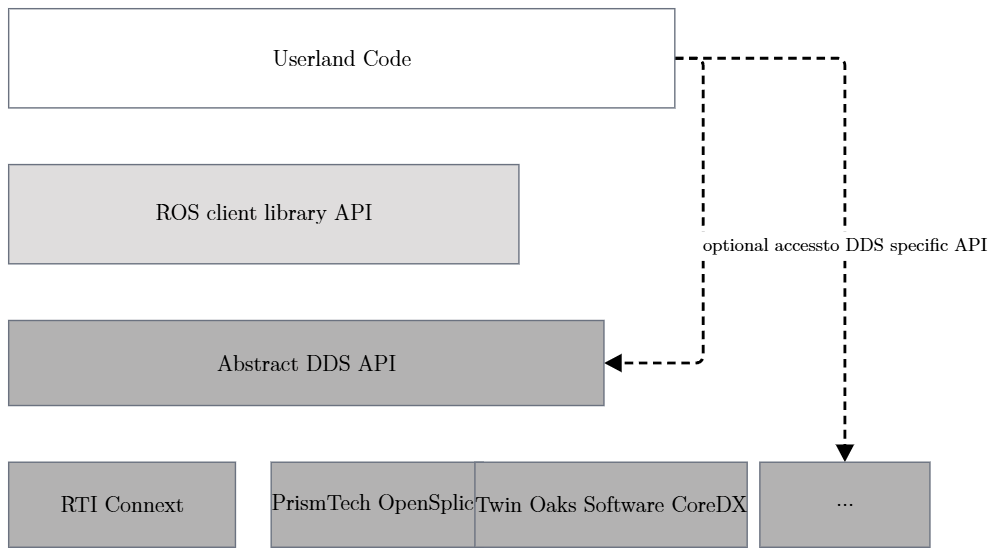
\includegraphics[width=0.8\textwidth]{figures/ROS2DDS架构.png}
  \caption{ROS2DDS架构}
  \label{fig:ROS2DDS架构}
\end{figure}

\section{ DDS 通信模型}
核心模型DCPS：以数据为中心的发布订阅。
DCPS模型通过主题实现发布者与订阅者的解耦，核心构成包括：
\begin{itemize}
    \item 域（Domain）：作为逻辑隔离的通信平面，只有相同域ID下的节点才能互相发现和通信，解决多系统同网络下的隔离问题。
    \item 主题（Topic）：是连接发布者与订阅者的逻辑纽带，对数据做分类标记，是发布和订阅匹配的唯一依据，发布者只需要发布对应主题的数据，所有订阅该主题的节点都会自动收到数据。
    \item 发布者/数据写入器（Publisher/DataWriter）：由发布者创建DataWriter，实际负责数据的发送。
    \item 订阅者/数据读取器（Subscriber/DataReader）：由订阅者创建DataReader，实际负责接收对应主题的数据。
\end{itemize}

这种模式下发布者和订阅者不需要知道对方的地址信息，仅通过主题完成匹配，能够轻松构建复杂的多对多通信关系，实现系统的高度解耦。

\section{ROS2的节点}
\subsection{使用g++编译ROS2节点}

程序编译一般需要经预处理、编译、汇编和链接几个步骤。在实际应用中，有些公共代码需要反复使用，就把这些代码编译成为“库”文件。在链接步骤中，链接器将从库文件取得所需的代码，复制到生成的可执行文件中，这种库称为静态（链接）库，其特点是可执行文件中包含了库代码的一份完整拷贝，缺点是被多次使用就会多份冗余拷贝。还有一种库，就是程序在开始运行后调用库函数时才被载入，这种库独立于现有的程序，其本身不可执行，但包含着程序需要调用的一些函数，这种库称为动态（链接）库\textit{（Dynamic Link Library）}。
\begin{figure}[htbp]
  \centering
  % ============================================================
% 从源文件到可执行程序的编译链接流程（由 Mermaid 流程图转写为 TikZ）
% 依赖：preamble.tex 中已加载的 tikz 宏包与 positioning、arrows.meta 库
% 用法：% ============================================================
% 从源文件到可执行程序的编译链接流程（由 Mermaid 流程图转写为 TikZ）
% 依赖：preamble.tex 中已加载的 tikz 宏包与 positioning、arrows.meta 库
% 用法：\input{figures/编译链接流程.tikz}（放在 figure 环境内，无需再写 \centering）
% 修改建议：改文字时请保持 text width 不变，否则底部说明可能自动换行错位
% ============================================================
\definecolor{cFlowRed}{HTML}{E74C3C}
\begin{tikzpicture}[
  font=\small,
  % 流程节点：红色边框、白底、圆角
  proc/.style={draw=cFlowRed, line width=1pt, rounded corners=1.5pt, fill=white,
               minimum height=0.75cm, minimum width=1.5cm, align=center,
               inner xsep=4pt, inner ysep=3pt},
  % 无边框文字（源文件、库文件、可执行文件、说明文字）
  txt/.style={align=center, inner sep=0pt},
  note/.style={align=left, inner sep=0pt, text width=11.5cm},
  % 流程箭头
  ar/.style={-{Stealth[length=2.2mm,width=2mm]}, line width=0.8pt, draw=black!80}
]

% ---------- 主干流程 ----------
\node[txt, anchor=west] (src) at (0,0) {源文件\\[-1pt]{\footnotesize (.h, .cpp 等)}};
\node[proc, right=6mm of src]  (pre)  {预编译};
\node[proc, right=6.5mm of pre] (comp) {编译};
\node[proc, right=6.5mm of comp] (asm)  {汇编};
\node[proc, right=6.5mm of asm]  (link) {链接};
\node[txt, right=6mm of link]   (exe)  {可执行文件};

% ---------- 链接阶段的外部输入：库文件 ----------
\node[txt, below=9mm of link] (lib) {.a / .lib\\[-1pt]{\footnotesize .so / .dll}};

% ---------- 用灰色虚线框标出“链接阶段” ----------
\draw[dashed, draw=black!45, line width=0.7pt]
  ([xshift=-3.2mm,yshift=-3.2mm]link.south west) rectangle
  ([xshift=3.2mm,yshift=3.2mm]link.north east);

% ---------- 连线 ----------
\draw[ar] (src) -- (pre);
\draw[ar] (pre) -- (comp);
\draw[ar] (comp) -- (asm);
\draw[ar] (asm) -- ([xshift=-3.2mm]link.west);
\draw[ar] (lib.north) -- ([yshift=-3.2mm]link.south);
\draw[ar] ([xshift=3.2mm]link.east) -- (exe);

% ---------- 底部说明文字 ----------
\node[note, anchor=north west] at (0,-2.9)
  {静态库、动态库的区别来自【链接阶段】如何处理库，\\
   链接成可执行程序，分别称为静态链接方式、动态链接方式。};
\end{tikzpicture}
（放在 figure 环境内，无需再写 \centering）
% 修改建议：改文字时请保持 text width 不变，否则底部说明可能自动换行错位
% ============================================================
\definecolor{cFlowRed}{HTML}{E74C3C}
\begin{tikzpicture}[
  font=\small,
  % 流程节点：红色边框、白底、圆角
  proc/.style={draw=cFlowRed, line width=1pt, rounded corners=1.5pt, fill=white,
               minimum height=0.75cm, minimum width=1.5cm, align=center,
               inner xsep=4pt, inner ysep=3pt},
  % 无边框文字（源文件、库文件、可执行文件、说明文字）
  txt/.style={align=center, inner sep=0pt},
  note/.style={align=left, inner sep=0pt, text width=11.5cm},
  % 流程箭头
  ar/.style={-{Stealth[length=2.2mm,width=2mm]}, line width=0.8pt, draw=black!80}
]

% ---------- 主干流程 ----------
\node[txt, anchor=west] (src) at (0,0) {源文件\\[-1pt]{\footnotesize (.h, .cpp 等)}};
\node[proc, right=6mm of src]  (pre)  {预编译};
\node[proc, right=6.5mm of pre] (comp) {编译};
\node[proc, right=6.5mm of comp] (asm)  {汇编};
\node[proc, right=6.5mm of asm]  (link) {链接};
\node[txt, right=6mm of link]   (exe)  {可执行文件};

% ---------- 链接阶段的外部输入：库文件 ----------
\node[txt, below=9mm of link] (lib) {.a / .lib\\[-1pt]{\footnotesize .so / .dll}};

% ---------- 用灰色虚线框标出“链接阶段” ----------
\draw[dashed, draw=black!45, line width=0.7pt]
  ([xshift=-3.2mm,yshift=-3.2mm]link.south west) rectangle
  ([xshift=3.2mm,yshift=3.2mm]link.north east);

% ---------- 连线 ----------
\draw[ar] (src) -- (pre);
\draw[ar] (pre) -- (comp);
\draw[ar] (comp) -- (asm);
\draw[ar] (asm) -- ([xshift=-3.2mm]link.west);
\draw[ar] (lib.north) -- ([yshift=-3.2mm]link.south);
\draw[ar] ([xshift=3.2mm]link.east) -- (exe);

% ---------- 底部说明文字 ----------
\node[note, anchor=north west] at (0,-2.9)
  {静态库、动态库的区别来自【链接阶段】如何处理库，\\
   链接成可执行程序，分别称为静态链接方式、动态链接方式。};
\end{tikzpicture}

  \caption{编译链接流程}
  \label{fig:编译链接流程}
\end{figure}
在widows平台下，静态链接库是.lib文件，动态库文件是.dll文件。在linux平台下，静态链接库是.a文件，动态链接库是.so文件。



\ifcsname wholebook\endcsname
\expandafter\endinput
\fi

% 单独编译模式: 在顶层(无未闭合条件)执行 \end{document} 收尾。
\end{document}

% 以后新增的章节文件, 请 \input 到对应分篇之下, 例如:
% \part{进阶篇}
% \input{ch03-ros2-install}

\end{document}
